\documentclass[journal]{IEEEtran}

% ---------------------------------------------------------------
% Packages
% ---------------------------------------------------------------
\usepackage{cite}
\usepackage{amsmath,amssymb,amsfonts}
\usepackage{graphicx}
\usepackage{textcomp}
\usepackage{xcolor}
\usepackage{booktabs}
\usepackage{multirow}
\usepackage{array}
\usepackage{url}
\usepackage{hyperref}
\usepackage{float}
\usepackage{placeins}

\graphicspath{{figures/}}

% Float spacing and placement tuning
\setlength{\textfloatsep}{8pt plus 2pt minus 4pt}
\setlength{\floatsep}{6pt plus 2pt minus 2pt}
\setlength{\intextsep}{8pt plus 2pt minus 2pt}
% Float placement. These govern how much of a page LaTeX may fill with floats.
% The earlier values (textfraction 0.07, topfraction 0.9) permitted pages that
% were almost entirely figures, which is what produced the figure-dump pages.
% textfraction is the key one: it is the minimum share of a page that must be
% body text before LaTeX is allowed to place a float there.
\renewcommand{\topfraction}{0.70}          % max share of a page top used by floats
\renewcommand{\bottomfraction}{0.45}
\renewcommand{\textfraction}{0.25}         % at least a quarter of the page must be text
\renewcommand{\floatpagefraction}{0.70}    % a float-only page must be 70% full to be allowed
\renewcommand{\dbltopfraction}{0.70}
\renewcommand{\dblfloatpagefraction}{0.70}
\setcounter{topnumber}{2}
\setcounter{bottomnumber}{1}
\setcounter{totalnumber}{3}
\setcounter{dbltopnumber}{1}                % at most one full-width float per page top

% ---------------------------------------------------------------
% Document
% ---------------------------------------------------------------
\begin{document}

\title{Evaluating the Predictive Utility of Synthetic Liver Cirrhosis Data for IoMT: A Comparative Study of Adversarial and Variational Architectures with Consensus-Based Quality Filtering}

\author{\IEEEauthorblockN{Michael~Udousoro\IEEEauthorrefmark{1},~Mohammad~Farhan~Khan\IEEEauthorrefmark{1},~Fakhreldin~Saeed\IEEEauthorrefmark{1},~and~M.~Mursaleen\IEEEauthorrefmark{2}}
\IEEEauthorblockA{\IEEEauthorrefmark{1}Department of Computing, School of Engineering, Computing and Design, University of Roehampton, London, United Kingdom}
\IEEEauthorblockA{\IEEEauthorrefmark{2}Department of Medical Research, China Medical University Hospital, China Medical University, Taichung, Taiwan}
\thanks{Manuscript submitted for review. \emph{(Corresponding author: Michael Udousoro, e-mail: michaeludousoro13@gmail.com.)}}}

\maketitle

% ---------------------------------------------------------------
% Abstract
% ---------------------------------------------------------------
\begin{abstract}
Clinical datasets stay small because of privacy rules and because some diseases are rare. The Mayo Clinic Primary Biliary Cirrhosis dataset shows this well: of 418 patient records, only 276 are complete. This study asks a simple question. Does adding synthetic records to the training data help a model predict outcomes better on real patients? During peer review we found a leakage problem and fixed it: N\_Days, the number of days a patient was followed up, had been used as an input feature. Since N\_Days is part of how the outcome itself is defined, this let the model see information it should not have had, and it inflated the reported baseline accuracy (AUC) from 0.842 to 0.878. Every result in this paper now excludes N\_Days from the model's inputs. We also test the problem three different ways, as plain classification of who eventually died, as classification of who died within three years, and as proper time-to-event survival modelling with Cox and Random Survival Forest models, so that our conclusions do not depend on one narrow way of framing the outcome.

We built three generative models from scratch in TensorFlow 2.15, using fixed random seeds throughout: a Vanilla GAN, a conditional GAN (cGAN), and a variational autoencoder (VAE). We also trained a masked-loss VAE on a larger, partially observed pool of patients, and a full CTGAN implementation, giving six generators in total. Every generated record passed a plausibility filter (an IQR-based Tukey fence), and a consensus step kept only the records that all three core models agreed looked realistic. We measured how well the synthetic data matched the real data using Fr\'{e}chet Inception Distance (FID) and a nearest-neighbour privacy check, and we measured whether it actually helped prediction using Random Forest, Gradient Boosting, and Logistic Regression classifiers (plus Cox and Random Survival Forest for the survival framing), tested with bootstrap confidence intervals, McNemar's exact test, and 5-fold cross-validation.

The masked-loss VAE had the best FID at 0.062, just ahead of cGAN's 0.072. The filtered adversarial pools were also reasonably private, with near-duplicate rates of 7.3\% and 9.6\%. Once we removed synthetic records from the validation folds, none of the augmentation methods, cGAN, consensus, or classic SMOTE oversampling, beat the real-data baseline by a significant margin. All McNemar p-values stayed above 0.06 across both the plain classification and the three-year framing. SMOTE showed a small cross-validation gain for Random Forest (0.856 versus 0.850), but this did not hold up under McNemar's test ($p = 0.063$). The survival framing told the same story for the Cox model, and gave a similar small, unproven gain for SMOTE under Random Survival Forest (0.867 versus 0.861). The one result worth stating plainly is the masked-loss VAE: augmenting with its larger training pool raised Random Forest AUC by 0.035 ($p = 0.125$). That is the closest this study came to a real effect, though it still falls short of significance at $n=83$. Consensus filtering did not lower privacy risk either, staying at 21.1\%, and its synthetic survival curve differs significantly from the real one ($p = 0.010$ by log-rank test) despite a mid-range FID.

A classifier trained only on cGAN data, with no real patients at all, still reached an AUC of 0.81 to 0.85 on real patients. This tells us synthetic data can carry real predictive signal, useful where real data cannot be shared, even when it cannot improve a dataset that is already large enough. Across all six generators, FID does not reliably predict how useful a generator's data turns out to be for training (Pearson $r = 0.35$, $p = 0.50$; Spearman $\rho = 0.26$, $p = 0.62$). In short, a generator that looks statistically similar to real data is not necessarily a generator whose data is useful for prediction.
\end{abstract}

\begin{IEEEkeywords}
Synthetic data generation, generative adversarial networks, variational autoencoder, liver cirrhosis, Internet of Medical Things, predictive utility, consensus voting, IQR filtering, patient privacy.
\end{IEEEkeywords}

% ---------------------------------------------------------------
% Section I: Introduction
% ---------------------------------------------------------------
\FloatBarrier
\section{Introduction}

Hospitals and clinics that use Internet of Medical Things (IoMT) devices continuously collect clinical measurements from wearable sensors and implanted monitoring devices. Biomarkers such as liver enzymes, bilirubin, albumin, and other laboratory measurements are automatically recorded and used by decision-support systems to help clinicians detect patient deterioration at an early stage \cite{guo2021}, \cite{obeid2023}. Machine learning models built from these records have already shown good performance in predicting mortality among patients with liver cirrhosis \cite{kanwal2020}.

For these systems to work reliably, they require large and well-labelled datasets, and obtaining such datasets is difficult. Privacy regulations such as GDPR and HIPAA restrict the sharing of patient information between healthcare institutions. In addition, rare diseases naturally produce small patient cohorts.

These two constraints bind particularly tightly in IoMT deployments. An IoMT decision-support system is rarely trained and deployed at the same site: a model developed at one hospital is expected to run at another, on that institution's own patients and its own devices. Pooling records across sites would solve the sample-size problem, but it is precisely what data protection law prevents. Synthetic data is attractive in this setting because it offers a way to move statistical structure between institutions without moving patient records, and it is this cross-site question, rather than augmentation in the abstract, that motivates the present study. The Mayo Clinic Primary Biliary Cirrhosis trial lasted more than ten years and collected 418 patient records from both a randomised trial and a later observational cohort. After removing records with missing measurements, only 276 complete cases remained \cite{fleming1991}, \cite{ucipbc}, making the development of a highly reliable classifier much more challenging.

Synthetic data generation offers a possible solution. Instead of sharing real patient records, a generative model learns the statistical patterns present in the training data and produces new records that appear realistic but do not belong to any actual patient \cite{goncalves2020}, \cite{gonzales2023}. GANs and VAEs have already been applied successfully in medical imaging, physiological time-series analysis, and tabular clinical datasets \cite{yan2022}, \cite{nikolentzos2023}, \cite{che2017}.

However, many previous studies have focused mainly on measuring how similar synthetic data is to real data, using metrics such as Fr\'{e}chet Inception Distance (FID) or Jensen-Shannon divergence. These metrics only measure similarity between distributions; they do not show whether synthetic data actually helps a classifier make better predictions on real patients. That practical question has received much less attention, especially for small tabular clinical datasets used in IoMT environments \cite{kababji2023}, \cite{espinosa2023}.

This study addresses that gap directly. The 276 complete PBC records were divided into 193 training patients and 83 held-out testing patients using a stratified 70/30 split with random seed 42. Three generative models were implemented from scratch in TensorFlow 2.15: a Vanilla GAN, a conditional GAN (cGAN) that generates records based on patient outcome labels, and a variational autoencoder (VAE).

Before the synthetic records were used for augmentation, two quality-control steps were applied. First, an IQR-based plausibility filter removed records with biomarker values outside the Tukey fence limits calculated from the real training data. Second, a consensus voting mechanism retained only the synthetic records that all three models placed in the same region of the feature space. The idea behind this approach is that agreement between different model architectures may provide a stronger indication of data quality than relying on a single model alone.

This work makes four main contributions:
\begin{enumerate}
  \item It provides a fair comparison of three structurally different generative models on the same liver cirrhosis dataset, all trained from scratch, extended to six generators for the synthetic-only evaluation in Section~\ref{sec:sixgen}.
  \item It introduces an IQR-based plausibility filter and a consensus voting mechanism as practical quality-control methods before augmentation.
  \item It evaluates synthetic augmentation using held-out real patients, 5-fold cross-validation, bootstrap confidence intervals, and McNemar's exact test, rather than relying only on distributional similarity metrics, and shows across six generators that FID does not significantly predict train-on-synthetic-test-on-real utility.
  \item It evaluates predictive utility under three framings, leakage-free binary classification, fixed-horizon landmark classification, and Cox/Random-Survival-Forest time-to-event modelling, so that the choice to binarise a censored outcome is not itself driving the conclusions.
\end{enumerate}

Section~\ref{sec:related} reviews related work. Section~\ref{sec:methodology} describes the dataset, models, and experimental design. Section~\ref{sec:results} presents the results, and Section~\ref{sec:conclusion} concludes.

% ---------------------------------------------------------------
% Section II: Related Work
% ---------------------------------------------------------------
\FloatBarrier
\section{Related Work}
\label{sec:related}

\subsection{Synthetic Data Generation for Healthcare}

Synthetic data generation is getting more attention as a way to share healthcare datasets without exposing real patients \cite{goncalves2020}, \cite{gonzales2023}, \cite{guillaudeux2023}. Many researchers now argue synthetic data should be judged not just on how well it protects privacy, but on how useful it actually is for real analysis. Gon\c{c}alves et al.\ reviewed methods for generating and evaluating synthetic patient data and argued this downstream utility deserves as much attention as privacy \cite{goncalves2020}. Gonzales et al.\ reviewed synthetic data in oncology, cardiology, and infectious disease, and flagged tabular electronic health records as an area still needing better generation methods \cite{gonzales2023}.

Older augmentation methods have real limits. SMOTE builds new minority-class samples by interpolating between existing records, so it cannot produce anything outside the range already present in the data \cite{kumari2024}, \cite{figueira2022}. Rule-based and statistical generators are easier to interpret but often miss the complex, non-linear relationships between clinical biomarkers. Deep generative models handle this better, since they learn those relationships directly from the data, and they are now one of the most common ways to generate synthetic clinical tabular data \cite{yan2022}, \cite{nikolentzos2023}.

\subsection{GAN Architectures for Tabular Clinical Data}

Generative Adversarial Networks work by training a generator and a discriminator against each other \cite{vega2020}. The generator tries to produce realistic synthetic records, while the discriminator attempts to distinguish synthetic records from real ones.

In healthcare applications, previous studies have shown that GAN-generated data can improve risk prediction using electronic health records \cite{che2017}. Choi et al.\ proposed medGAN for generating multi-label patient records, showing that GAN-based approaches can be useful for clinical data synthesis \cite{choi2017}. However, standard GANs often experience mode collapse and unstable training when applied to tabular clinical datasets containing a mixture of continuous variables, binary indicators, and ordinal disease-stage variables \cite{lenz2021}, \cite{espinosa2023}.

The conditional GAN was developed to reduce some of these problems by conditioning both the generator and the discriminator on a class label, which helps ensure that minority classes are represented more fairly during training \cite{vega2020}, \cite{sharma2024}. The variational autoencoder uses a different strategy. Instead of adversarial training, it learns a latent representation of patient records through an encoder-decoder structure, and new patient records are generated at inference time by sampling from that latent space \cite{nikolentzos2023}.

\subsection{Synthetic Data for IoMT}

IoMT systems continuously collect physiological measurements from connected medical devices, and these systems require large labelled datasets to support reliable machine learning models \cite{guo2021}, \cite{obeid2023}.

Previous studies have shown that synthetic data can improve anomaly detection in IoMT environments \cite{meidan2018}. Other researchers have demonstrated that synthetic patient cohorts can support research in diseases where the number of available real patients is very small \cite{damico2023}. Synthetic augmentation has also been reported to improve survival prediction in rare-disease tabular datasets similar in nature to the PBC dataset used in this study \cite{kim2024}. In addition, high-quality synthetic patient data has been shown to be useful for testing healthcare software systems, provided that the quality of the generated data is carefully evaluated \cite{tucker2020}.

\subsection{From Distributional Fidelity to Predictive Utility}

Most evaluation approaches so far focus on distributional fidelity, how closely synthetic data resembles real data, using metrics like FID, Jensen-Shannon divergence, or Kolmogorov-Smirnov statistics \cite{yan2022}, \cite{figueira2022}, \cite{dankar2022}. But good distributional similarity does not guarantee good predictive performance. Espinosa and Figueira found the link between distributional metrics and downstream utility is often weak \cite{espinosa2023}. Foraker et al.\ reported that synthetic data can give different analytical results than the real data it was built from, even when it looks highly realistic \cite{foraker2020}.

Kababji et al.\ argued a more meaningful test is whether models trained on synthetic data can reproduce clinically important findings from real patients \cite{kababji2023}. Kaabachi et al.\ pointed to a lack of evaluation on fully held-out real patients as a major weakness across many medical synthetic-data studies \cite{kaabachi2023}. That is exactly why we designed this study to test predictive utility on unseen real patients, not just similarity metrics.

\subsection{Multi-Model Ensemble Strategies and the Positioning of This Work}

Some previous studies have explored the idea of combining the outputs of multiple generative models. Jiang et al.\ proposed a multi-source augmentation framework in which several GAN models are trained independently and their outputs are combined to improve data quality \cite{jiang2023}. The consensus voting method used in this study is related to that idea, but differs in two important ways. First, it uses three different generative architectures rather than several versions of the same GAN. Second, a synthetic record is accepted only when there is agreement across all three models, instead of simply merging all generated records together.

Within the IoMT field, Pandey et al.\ introduced MF-CGAN, which generates synthetic network traffic and health-related measurements by conditioning on multiple variables \cite{pandey2025}. The present work differs because it focuses on clinical tabular data containing continuous laboratory biomarkers, ordinal disease stages, and binary clinical indicators measured during a single patient visit.

Another important difference is the evaluation strategy. In this study, classifiers are trained on augmented datasets but tested only on real held-out patients. The results show that the proposed consensus voting method did not improve prediction accuracy, cross-validation stability, or disclosure risk for this small clinical dataset. Although this is a negative result, it is still valuable because it provides useful evidence for the design of future synthetic-data augmentation pipelines.

% ---------------------------------------------------------------
% Section III: Methodology
% ---------------------------------------------------------------
\FloatBarrier
\section{Methodology}
\label{sec:methodology}

\subsection{Dataset and Preprocessing}

The dataset used in this study is the Mayo Clinic Primary Biliary Cirrhosis (PBC) trial \cite{fleming1991}, obtained from the UCI Machine Learning Repository \cite{ucipbc}. The raw file contains 418 patient records and 20 columns. The patient identifier column carries no clinical information and is discarded. The remaining 19 columns consist of 11 continuous laboratory measurements (N\_Days, Age, Bilirubin, Cholesterol, Albumin, Copper, Alk\_Phos, SGOT, Triglycerides, Platelets, and Prothrombin), five binary clinical indicators (Sex, Drug, Ascites, Hepatomegaly, and Spiders), two ordinal variables (Edema coded as 0~=~none, 1~=~slight/suspected, 2~=~confirmed; Stage coded 1--4), and the binary survival outcome Status (0~=~censored/transplanted, 1~=~deceased).

Patients 313--418 belong to an observational cohort missing between 9 and 10 laboratory measurements each. Rather than imputing values collected under fundamentally different protocols (which would introduce systematic bias), complete-case analysis is applied: any row containing at least one missing value is removed, yielding 276 complete patient records. Categorical columns are numerically encoded: Sex (Female~=~0, Male~=~1), Drug (Placebo~=~0, D-penicillamine~=~1), Ascites/Hepatomegaly/Spiders (No~=~0, Yes~=~1), and Status (censored/transplanted~=~0, deceased~=~1). All features are then scaled to $[0, 1]$ using a MinMaxScaler fitted exclusively on the training partition to prevent data leakage. The Pearson correlation structure across all 276 complete cases is given in Fig.~S1; Bilirubin and N\_Days emerge as the most clinically informative axes, with Bilirubin correlating positively with Copper ($r = 0.46$) and SGOT ($r = 0.42$), and N\_Days correlating negatively with Bilirubin ($r = -0.43$).

The 276 records are divided into a training set of 193 patients and a held-out test set of 83 patients using stratified random splitting with seed 42, preserving class balance in both partitions (training: 115 survived/transplanted = 59.6\%, 78 deceased = 40.4\%). The overall pipeline (Fig.~S16 in the supplementary document) takes the raw 418-patient dataset through a complete-case filter and preprocessing, then feeds the 193-patient training set to three parallel generative models, each passing its 500 generated records through the IQR filter before all three filtered pools enter consensus voting.

\subsection{Generative Model Architectures}

All three models are implemented from scratch in TensorFlow 2.15 without third-party synthetic data libraries. Each model receives the MinMax-scaled training data and produces samples in the same normalised $[0, 1]$ range, which are inverse-transformed to recover original clinical units after generation. Each model generates 500 synthetic records.

\textbf{Vanilla GAN.} The generator maps a 100-dimensional noise vector $\mathbf{z}$ drawn from a standard normal distribution through two dense hidden layers of 128 and 256 units with Leaky ReLU activations ($\alpha = 0.2$) and batch normalisation (momentum~$= 0.8$) to a sigmoid output of dimension 18. The discriminator maps each patient record through two dense layers of 256 and 128 units with Leaky ReLU activations and dropout ($p = 0.3$). Both networks use the Adam optimiser with learning rate $2 \times 10^{-4}$ and $\beta_1 = 0.5$ for 500 epochs at batch size 32. The adversarial objectives are:
\begin{align}
\mathcal{L}_D &= -\mathbb{E}[\log D(\mathbf{x})] - \mathbb{E}[\log(1 - D(G(\mathbf{z})))] \\
\mathcal{L}_G &= -\mathbb{E}[\log D(G(\mathbf{z}))]
\end{align}

\textbf{Conditional GAN (cGAN).} This model extends the Vanilla GAN by conditioning both generator and discriminator on the patient outcome label $\mathbf{y}$, supplied as a two-dimensional one-hot vector. It follows Mirza and Osindero \cite{mirza2014} rather than the Conditional Tabular GAN (CTGAN) of Xu et al.\ \cite{xu2019}, and we name it accordingly: it adopts the idea of conditioning generation on an outcome label, but implements none of the three components that define CTGAN, namely mode-specific normalisation, training-by-sampling, and a PacGAN critic trained with the Wasserstein gradient penalty. Section~\ref{sec:ctgancomp} reports a direct comparison against a full CTGAN implementation on this cohort. The generator receives the concatenation $[\mathbf{z} \| \mathbf{y}]$, and the discriminator receives $[\mathbf{x} \| \mathbf{y}]$. Training uses balanced mini-batches, drawing equal numbers of survivors and deceased patients at each step. Architecture and optimiser settings match the Vanilla GAN, with training for 300 epochs.

\textbf{Variational Autoencoder (VAE).} This is a standard variational autoencoder applied to the min-max scaled table. As with the cGAN, we name it for what it is: it is not the TVAE of Xu et al.\ \cite{xu2019}, which additionally applies mode-specific normalisation, and results reported here should not be read as a benchmark of that model. The encoder maps each patient record through two dense layers of 128 and 64 units with ReLU activations to a mean vector $\boldsymbol{\mu}$ and log-variance vector $\log(\boldsymbol{\sigma}^2)$ of dimension 32. A latent sample is drawn using the reparameterisation trick:
\begin{equation}
\mathbf{z} = \boldsymbol{\mu} + \boldsymbol{\varepsilon} \cdot \exp(0.5 \cdot \log(\boldsymbol{\sigma}^2)),
\end{equation}
where $\boldsymbol{\varepsilon}$ is drawn from a standard normal. The decoder maps $\mathbf{z}$ through two dense layers of 64 and 128 units with ReLU activations to a sigmoid output of dimension 18. The training objective is the Evidence Lower Bound (ELBO):
\begin{equation}
\mathcal{L}_{\text{VAE}} = \mathbb{E}\!\left[\|\mathbf{x} - \hat{\mathbf{x}}\|^2\right] + \beta \cdot D_{\text{KL}}\!\left(\mathcal{N}(\boldsymbol{\mu}, \boldsymbol{\sigma}^2) \,\|\, \mathcal{N}(\mathbf{0}, \mathbf{I})\right)
\end{equation}
with $\beta = 1.0$, Adam optimiser at learning rate $1 \times 10^{-3}$, batch size 32, and 300 training epochs. Training loss curves for all three models are given in Fig.~S2. The adversarial losses settle without the oscillation that signals mode collapse, and the VAE ELBO falls sharply before levelling off by roughly epoch 50, so all three models are trained to convergence.

\subsection{IQR-Based Physiological Plausibility Filter}

A Tukey fence filter is applied independently to each model's output. For each of the 11 continuous clinical features, the first and third quartiles, $Q_1$ and $Q_3$, are computed from the real training set alone. A synthetic record is retained only if every continuous feature value falls within $[Q_1 - 1.5 \times \text{IQR},\; Q_3 + 1.5 \times \text{IQR}]$. A single out-of-range value disqualifies the entire record. Binary and ordinal features are exempt because they are snapped to valid integer ranges during post-processing.

Applied to 500 generated records per model, the filter retained 331 GAN records (66.2\%), 292 cGAN records (58.4\%), and 499 VAE records (99.8\%). Fig.~S13 in the supplementary document illustrates the effect on the Bilirubin distribution, the most challenging continuous feature to reproduce faithfully.

\subsection{Multi-Method Consensus Voting}

A consensus voting mechanism is applied that retains only records independently corroborated by all three generative models. This approach is related to the multi-source data augmentation strategy of Jiang et al.\ \cite{jiang2023}, who combine outputs from multiple independently trained GANs to reduce distribution skewness. The present work differs in that three structurally distinct architectures are used, and acceptance requires cross-architecture agreement rather than simply pooling all outputs.

A StandardScaler is fitted on the union of all three filtered datasets. For each candidate record from one model, the minimum Euclidean distance to any record from each of the other two models is computed in standardised space. The candidate is accepted if both other models have a record within tolerance~$= 5.0$ standardised units. This process repeats with each filtered dataset as the candidate pool in turn, and exact duplicates are removed from the final set. The threshold of 5.0 was selected on the basis of a systematic sensitivity analysis conducted across eight values from 2.5 to 6.0. At thresholds of 3.0 and below, the accepted set contains around 10\% deceased patients or fewer, a severe class imbalance relative to the real training cohort (40\% deceased). As the tolerance increases the deceased fraction recovers (24.7\% at 5.0) and the FID score falls monotonically (0.095 at 5.0), after which further increases yield only marginal FID improvements (0.0864 at 5.5, 0.0829 at 6.0) while admitting records with progressively weaker cross-model agreement. The value of 5.0 therefore represents the point at which class balance becomes acceptable and the quality improvement curve begins to flatten. To address the pool-size imbalance across the three filtered datasets (GAN 331 records, cGAN 292 records, VAE 499 records), the VAE pool is randomly downsampled to 292 records before voting, matching the size of the smallest adversarial pool. This equalisation gives the two higher-fidelity adversarial models a proportionally stronger role in the consensus. The equalised consensus of 787 records achieves FID 0.0809, with source composition GAN 33.2\%, cGAN 29.7\%, and VAE 37.1\%.

\subsection{Synthetic Data Quality Evaluation}

Distributional fidelity is assessed using a tabular proxy Fr\'{e}chet Inception Distance computed on the 18-dimensional feature vectors:
\begin{equation}
\text{FID} = \|\boldsymbol{\mu}_r - \boldsymbol{\mu}_s\|^2 + \text{Tr}\!\left(\boldsymbol{\Sigma}_r + \boldsymbol{\Sigma}_s - 2(\boldsymbol{\Sigma}_r \boldsymbol{\Sigma}_s)^{1/2}\right).
\end{equation}
Lower values indicate greater distributional alignment. Per-feature Kolmogorov-Smirnov tests, Jensen-Shannon divergence, Cohen's $d$, Shapiro-Wilk normality tests, and chi-square tests for categorical features provide a granular distributional profile. Privacy risk is assessed through nearest-neighbour distance analysis. For each synthetic record, the Euclidean distance to the closest real training patient is computed in StandardScaler-normalised feature space across all 18 input features. A record is flagged as a near-duplicate if its distance falls below the 5th percentile of real-to-real nearest-neighbour distances, a data-driven threshold that identifies synthetic records closer to any real patient than 95\% of real patients are to their nearest real neighbour.

\subsection{Predictive Utility Evaluation}
\label{sec:predutil}

N\_Days is the number of days from registration to whichever comes first, death, transplant, or the end of the study. It is the follow-up duration, defined jointly with Status, not something measured at enrolment. Using it as a classifier input leaks the outcome, because a short N\_Days is tied to a recorded death simply by how it is built. So every classifier in this section trains on the remaining 17 features, with N\_Days left out. Every synthetic-data model still generates N\_Days, since we need it for the landmark and survival framings in Sections~\ref{sec:landmark} and~\ref{sec:survival}, but no classifier predicting Status ever sees it.

Predictive utility is evaluated by training Random Forest (RF), Gradient Boosting (GB), and Logistic Regression (LR) classifiers under five training scenarios and testing on the 83-patient held-out real test set:
\begin{itemize}
  \item \textbf{Scenario A:} 193 real patients only (baseline).
  \item \textbf{Scenario B:} 193 real + IQR-filtered cGAN records. cGAN is selected here because it achieves the lowest FID among the three individual generators trained from scratch (Section~\ref{sec:results}).
  \item \textbf{Scenario C:} 193 real + consensus records.
  \item \textbf{Scenario D:} 193 real patients augmented with SMOTE oversampling (classical baseline).
  \item \textbf{Scenario E:} IQR-filtered synthetic records only, with no real patients in training (synthetic-only, train-on-synthetic-test-on-real). Section~\ref{sec:sixgen} extends this scenario from cGAN alone to all six generators available in this study (Vanilla GAN, cGAN, VAE, a masked-loss VAE trained on a larger partially observed pool, a full CTGAN implementation, and consensus), so that FID can be checked against downstream utility across more than one point.
\end{itemize}
The classifiers use fixed configurations (Random Forest and Gradient Boosting with 200 estimators, Gradient Boosting depth 3, Logistic Regression with 1000 iterations) applied identically across all scenarios so the comparison is fair. Evaluation metrics are Accuracy, F1, Precision, Recall, and AUC-ROC. Five-fold stratified cross-validation, 1000-resample bootstrap confidence intervals, and McNemar's exact test complement the single-split evaluation. In cross-validation the folds are drawn from the real training patients only; synthetic records are added exclusively to the training side of each fold and every validation fold contains real patients alone, so no synthetic record ever leaks into validation. All random seeds are fixed at 42, and the generative models are trained under fixed Python, NumPy, and TensorFlow seeds so the full pipeline is reproducible.

\subsection{Fixed-Horizon Landmark Classification}
\label{sec:landmark}

Coding Status as censored-or-transplanted~=~0 versus deceased~=~1 throws away timing information: a patient censored at 400 days and one censored at 4{,}500 days get the same code, even though the first tells us almost nothing about long-run survival and the second tells us a lot. So as a leak-free alternative that still fits a normal classification setup, we also test a fixed 3-year landmark. A patient is labelled an event if death happened within 3 years (1,095.75 days) of registration, and a survivor if they were followed for at least 3 years without dying, whatever happens after that. A patient censored or transplanted \emph{before} 3 years is dropped rather than counted as a survivor, because we genuinely do not know their status at the landmark; counting them either way would just bring back the same censoring problem we are trying to avoid. We apply this same rule to real and synthetic records alike, using each record's own N\_Days and Status, so both are labelled the same consistent way. At the 3-year mark, 187 of 193 real training patients and 76 of 83 real test patients are usable. We re-run Scenarios A-E on this horizon-filtered, relabelled cohort, using the same 17-feature input as Section~\ref{sec:predutil}.

\subsection{Time-to-Event Survival Modelling}
\label{sec:survival}

The landmark framing avoids coding a censored-before-horizon patient as a survivor, but it still throws away the exact timing of events past the horizon. As a more direct alternative, we fit a Cox proportional-hazards model (duration~=~N\_Days, event~=~Status, covariates~=~the same 17 features, ridge penalizer~$=0.1$), and, where scikit-survival is available, a Random Survival Forest (200 trees, minimum leaf size 3), both evaluated with Harrell's concordance index (C-index) on the real held-out test set. No horizon choice is needed here, since we use each patient's full follow-up time directly, whether or not their event was observed.

We code death as the event (1) and both staying alive and getting a transplant as non-events (0). This is a cause-specific hazard for death, not a formal competing-risks model, and it assumes transplant timing tells us nothing extra about death risk beyond what the covariates already capture. Transplant is a genuine competing risk, not ordinary loss to follow-up, so treating it as the latter is a modelling choice, not something we can just assume is fine. We checked how big a concern this really is. Fig.~S11 in the supplementary document plots the non-parametric Aalen-Johansen cumulative incidence of death versus transplant, which does not need that non-informative-censoring assumption at all. Of the 276 complete-case patients, 111 (40.2\%) died and only 18 (6.5\%) were transplanted, and the cumulative incidence of transplant stays under 9\% throughout follow-up against 64\% for death. So the competing event is rare enough that censoring at transplant is unlikely to seriously bias our results. Stating that precisely rather than just qualitatively would need a full competing-risks regression, for example a Fine-Gray model, which no package in our pipeline currently supports, so we did not fit one here.

Scenarios A-E mirror the classification framing, pooling real and synthetic records into one training set before fitting. Scenario D needs a caveat: standard SMOTE has no concept of a censored duration target, since it interpolates a feature vector between a minority-class record and a same-class neighbour, and that is not well defined when the label itself might be a censored time. So we use a documented substitute instead: for each event~=~1 (deceased) record, we find a same-class nearest neighbour in standardised covariate space, and build a synthetic record by interpolating both the covariates and N\_Days by the same random weight, keeping event~=~1, until the event class matches the censored class in size, exactly as classical SMOTE would balance it. We say this explicitly because it is a deviation from off-the-shelf SMOTE, not an equivalent stand-in.

We also compare each generator's synthetic (N\_Days, Status) distribution against the real training cohort using Kaplan-Meier curves and a log-rank test. This checks whether a generator reproduces the time-to-event structure specifically, something FID (computed over the full 18-dimensional feature space) does not tell us on its own.

% ---------------------------------------------------------------
% Section IV: Results and Discussion
% ---------------------------------------------------------------
\FloatBarrier
\section{Results and Discussion}
\label{sec:results}

\subsection{Synthetic Data Retention and IQR Filtering}

Table~\ref{tab:retention} summarises IQR filter retention rates and FID scores. The GAN and cGAN each reject roughly one third to one half of their generated records; the VAE retains almost all. The consensus procedure accepts 787 records from the equalised filtered pools (VAE downsampled to 292).

\begin{table}[!tb]
  \centering
  \caption{Synthetic Data Retention and FID Scores}
  \label{tab:retention}
  \begin{tabular}{lcccc}
    \toprule
    Method & Generated & Retained & Retention & FID \\
    \midrule
    Vanilla GAN   & 500 & 331 & 66.2\% & 0.0995 \\
    cGAN         & 500 & 292 & 58.4\% & 0.0724 \\
    VAE          & 500 & 499 & 99.8\% & 0.2280 \\
    Consensus     & ---  & 787 & ---   & 0.0809 \\
    \bottomrule
  \end{tabular}
\end{table}

\subsection{Distributional Fidelity}

Table~\ref{tab:retention} already gives the FID scores for all four synthetic datasets. cGAN has the lowest FID at 0.0724, followed by the Vanilla GAN at 0.0995. The VAE reaches an FID of 0.2280 despite keeping almost all its generated records, which confirms that smooth variational generation loses distributional sharpness. The equalised consensus set scores 0.0809.

Three further views support this ranking and are provided as supplementary material. Fig.~S3 compares feature distributions for six representative clinical variables: Albumin and Prothrombin are well reproduced by GAN and cGAN, while Bilirubin is the hardest feature, with the VAE distribution shifted noticeably rightward relative to real patients. Fig.~S4 compares the Pearson correlation structure of real and consensus data, showing that the consensus set preserves the dominant pairwise associations, including the positive Bilirubin-Copper and negative N\_Days-Bilirubin relationships, though weaker correlations are attenuated. Fig.~S5 gives a t-SNE projection in which the GAN and cGAN sets mix with the real patient manifold, the VAE points spread beyond the real density contours, and the consensus set concentrates in the central high-density region.

Per-feature KS tests show a consistent pattern. The filtered GAN shows no significant distributional difference from real training data on Age (KS~$= 0.083$, $p = 0.348$), Triglycerides (KS~$= 0.081$, $p = 0.380$), and Prothrombin (KS~$= 0.092$, $p = 0.234$), but diverges significantly on Bilirubin (KS~$= 0.413$), Alk\_Phos (KS~$= 0.506$), and Cholesterol (KS~$= 0.308$). The VAE diverges significantly on all 11 continuous features. The consensus set achieves substantially smaller KS statistics on the most challenging biomarkers: Bilirubin KS~$= 0.269$ vs.\ GAN's 0.413; Alk\_Phos KS~$= 0.249$ vs.\ GAN's 0.506.

\subsection{Privacy Risk Assessment}

We assess privacy risk using nearest-neighbour distances in standardised feature space (full violin plots in Fig.~S14 of the supplementary document). The GAN and cGAN distributions sit well above the risk threshold (5th percentile of real-to-real distances), so most adversarially generated records fall at a safe distance from any real patient. The VAE and consensus distributions have substantial mass below the threshold, reflecting the broader coverage of the variational latent space and the fact that consensus acceptance pools records lying close to real patients. Table~\ref{tab:privacy} gives the near-duplicate rates and mean nearest-neighbour distances for each method. Consensus voting does not improve on the individual adversarial pools. At a 21.1\% near-duplicate rate it is far riskier than the filtered GAN (7.3\%) or cGAN (9.6\%), because it inherits the VAE records that sit closest to real patients.

\begin{table}[!tb]
  \centering
  \caption{Privacy Risk Analysis}
  \label{tab:privacy}
  \begin{tabular}{lcccc}
    \toprule
    Method & Records & Mean Dist. & Near-Dup. & Rate \\
    \midrule
    GAN (filtered)   & 331 & 2.23 & 24  & 7.3\%  \\
    cGAN (filtered) & 292 & 2.34 & 28  & 9.6\%  \\
    VAE (filtered)  & 499 & 1.60 & 178 & 35.7\% \\
    Consensus        & 787 & 1.91 & 166 & 21.1\% \\
    \bottomrule
  \end{tabular}
\end{table}

\subsection{Predictive Utility on the Held-Out Test Set}

Table~\ref{tab:performance} reports complete test-set metrics across all five scenarios.

\begin{table*}[t]
  \centering
  \caption{Test-Set Classification Performance, N\_Days Excluded from Classifier Input (83 Real Held-Out Patients)}
  \label{tab:performance}
  \begin{tabular}{llccccccc}
    \toprule
    Scenario & Classifier & $n_{\text{train}}$ & Accuracy & F1 & Precision & Recall & AUC \\
    \midrule
    A: Baseline       & Random Forest      & 193 & 0.7831 & 0.7848 & 0.7901 & 0.7831 & 0.8324 \\
    A: Baseline       & Gradient Boosting  & 193 & 0.7831 & 0.7848 & 0.7901 & 0.7831 & 0.8297 \\
    A: Baseline       & Logistic Regression& 193 & 0.8193 & 0.8204 & 0.8237 & 0.8193 & \textbf{0.8424} \\
    \midrule
    B: Real + cGAN   & Random Forest      & 485 & 0.7831 & 0.7848 & 0.7901 & 0.7831 & 0.8370 \\
    B: Real + cGAN   & Gradient Boosting  & 485 & 0.7952 & 0.7965 & 0.7998 & 0.7952 & 0.8085 \\
    B: Real + cGAN   & Logistic Regression& 485 & 0.7590 & 0.7614 & 0.7716 & 0.7590 & 0.8467 \\
    \midrule
    C: Real + Consensus & Random Forest    & 980 & 0.7590 & 0.7614 & 0.7716 & 0.7590 & 0.8321 \\
    C: Real + Consensus & Gradient Boosting& 980 & 0.7108 & 0.7139 & 0.7301 & 0.7108 & 0.8176 \\
    C: Real + Consensus & Logistic Regression & 980 & 0.8193 & 0.8211 & 0.8346 & 0.8193 & 0.8461 \\
    \midrule
    D: Real + SMOTE   & Random Forest      & 230 & \textbf{0.7952} & \textbf{0.7965} & 0.7998 & 0.7952 & 0.8191 \\
    D: Real + SMOTE   & Gradient Boosting  & 230 & 0.7590 & 0.7614 & 0.7716 & 0.7590 & 0.8339 \\
    D: Real + SMOTE   & Logistic Regression& 230 & 0.7590 & 0.7616 & 0.7782 & 0.7590 & 0.8358 \\
    \midrule
    E: Synthetic Only (cGAN) & Random Forest      & 292 & 0.6867 & 0.6840 & 0.7672 & 0.6867 & 0.8091 \\
    E: Synthetic Only (cGAN) & Gradient Boosting  & 292 & 0.6506 & 0.6506 & 0.7076 & 0.6506 & 0.6867 \\
    E: Synthetic Only (cGAN) & Logistic Regression& 292 & 0.6988 & 0.6988 & 0.7600 & 0.6988 & 0.8485 \\
    \bottomrule
  \end{tabular}
\end{table*}

Fig.~\ref{fig:roc} shows the ROC curves for all three classifiers across scenarios A, B and C on the 83-patient real held-out test set, now trained on the 17-feature leak-free input. All curves lie substantially above the random classifier diagonal. With N\_Days excluded, the highest baseline AUC drops from Gradient Boosting to Logistic Regression at 0.842 (Gradient Boosting falls from 0.878 to 0.830). Logistic Regression under Scenario B nominally exceeds this at 0.847, and under Scenario C at 0.846, but both sit well inside the overlapping bootstrap intervals in Table~\ref{tab:significance} and neither McNemar comparison reaches significance (Table~\ref{tab:significance}), so this is noise rather than a real augmentation effect.

\begin{figure*}[!t]
  \centering
  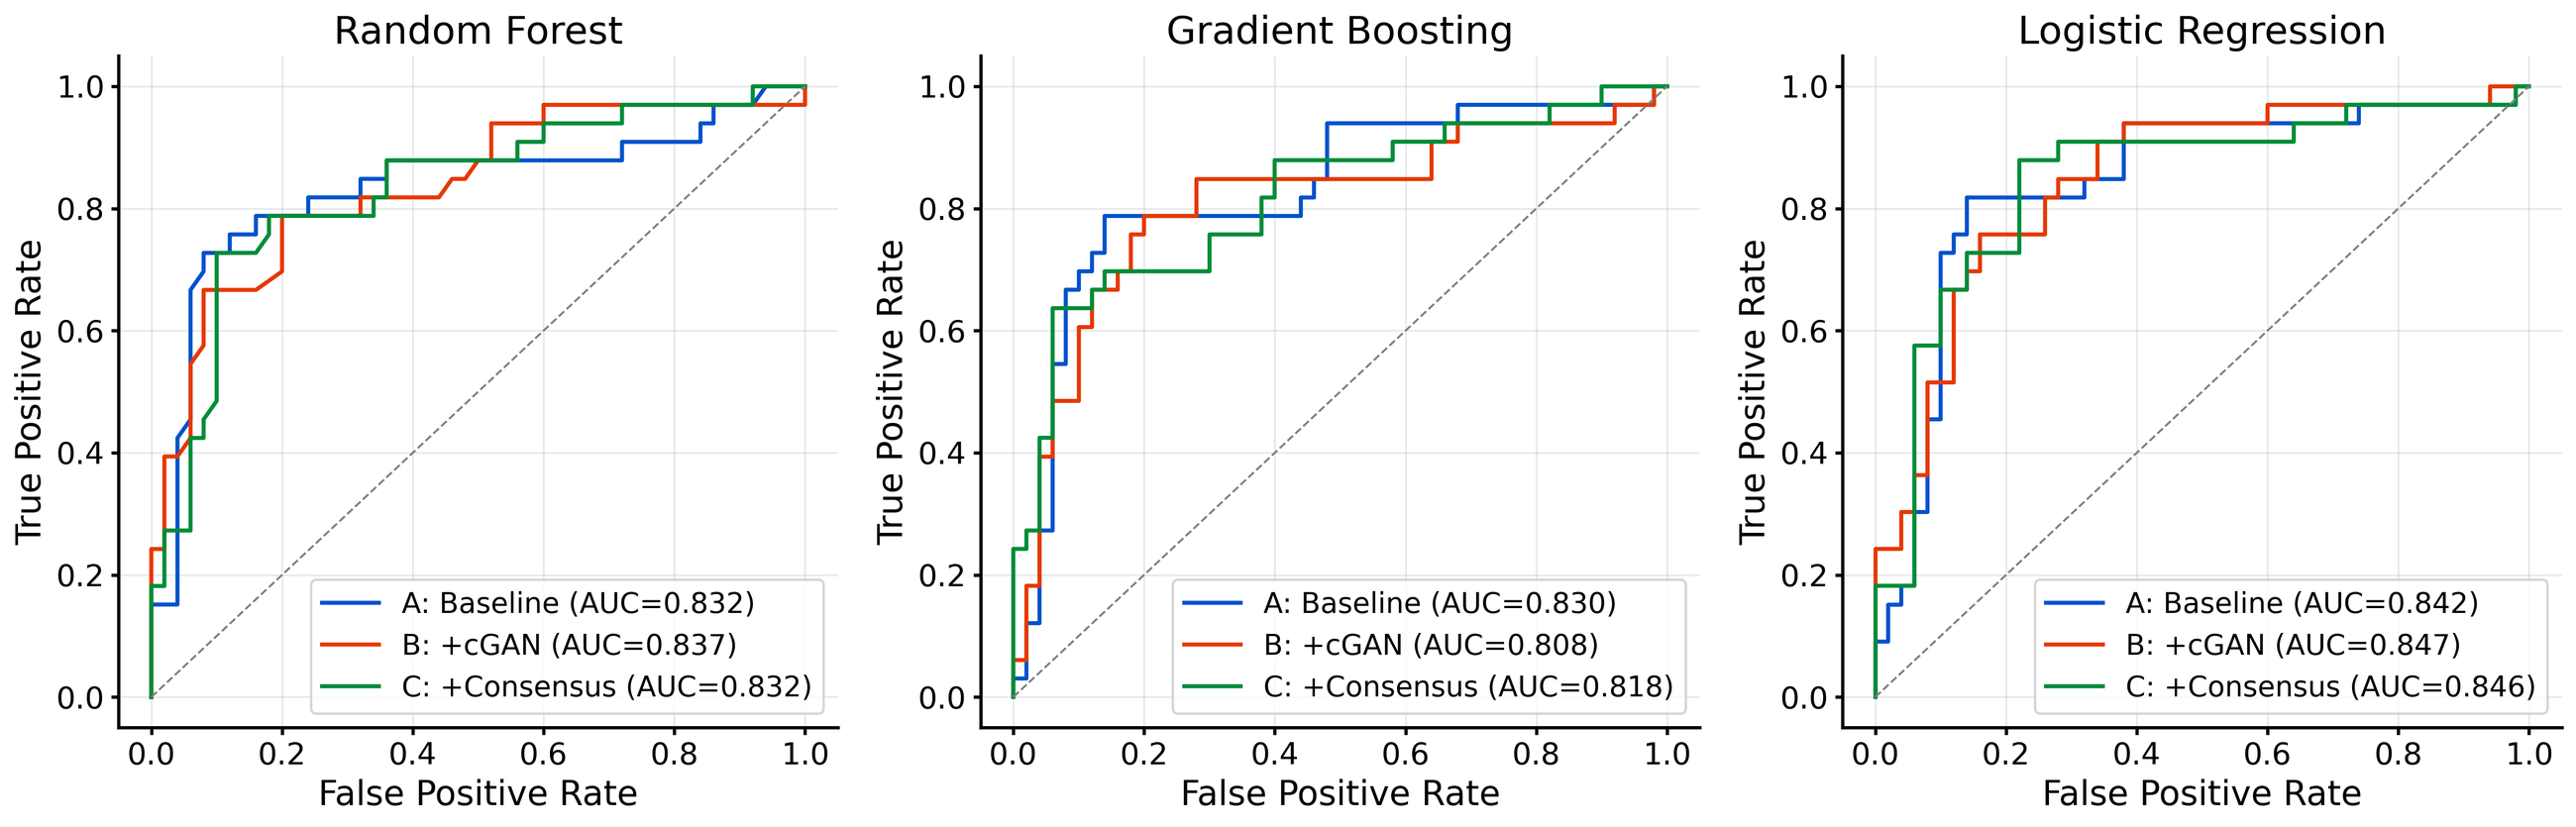
\includegraphics[width=0.98\textwidth]{fig06_roc_curves.png}
  \caption{ROC curves by classifier and training scenario on the 83-patient real held-out test set, N\_Days excluded from classifier input: Random Forest (left), Gradient Boosting (centre), Logistic Regression (right). All curves lie substantially above the random classifier diagonal. The highest baseline AUC is now Logistic Regression at 0.842; Gradient Boosting's baseline AUC falls from 0.878 (N\_Days included) to 0.830 once the leaked feature is removed.}
  \label{fig:roc}
\end{figure*}

Because all of these numbers appear in Table~\ref{tab:performance}, the corresponding graphical views are supplied as supplementary material rather than repeated here. Fig.~S6 gives Precision-Recall curves, which matter for this cohort given its class imbalance, and shows precision holding above 0.7 across a wide recall range for every classifier. Fig.~S7 plots AUC across scenarios, Fig.~S8 gives the F1 heatmap, and Figs.~S9 and~S10 compare all five metrics across scenarios. The pattern across all of them is the same: every scenario and classifier combination clears AUC~$= 0.8$, so no augmentation strategy damages discrimination, but none uniformly improves on the baseline either. Gradient Boosting is the only classifier whose F1 falls monotonically as synthetic volume increases from Scenario A to C.

\subsection{Cross-Validation}

Table~\ref{tab:cv} presents 5-fold stratified cross-validation AUC results, computed with synthetic records confined to the training side of each fold and every validation fold containing real patients only, on the leak-free 17-feature input. Under this protocol, neither deep-generative augmentation scenario (B or C) improves the mean cross-validated AUC over the real-data baseline for Random Forest or Gradient Boosting; both lower the mean for these two classifiers while marginally raising it for Logistic Regression (0.8357 and 0.8349 against a baseline of 0.8321). SMOTE (Scenario D) is a partial exception, worth stating plainly rather than folding into the same null result as B and C: it raises the Random Forest mean to 0.8559, above the baseline's 0.8499, while lowering Gradient Boosting to 0.8126 and leaving Logistic Regression essentially unchanged (0.8300). This is the same pattern the reviewer identified in the pre-correction numbers, now confirmed on the leak-free feature set: a classical interpolation baseline can nominally beat real-data-only training on a subset of classifiers, even though no deep-generative scenario does. The fold-to-fold standard deviation shows no consistent direction either: Gradient Boosting falls modestly from 0.0535 (Scenario A) to 0.0480 (Scenario C), while Random Forest rises from 0.0464 to 0.0532 over the same comparison. This is a different picture from an earlier, since-corrected version of this analysis, in which allowing synthetic records into the validation folds produced a large apparent variance reduction; no such effect appears once validation is restricted to real patients, with or without N\_Days as a feature.

\begin{table}[!tb]
  \centering
  \caption{5-Fold Cross-Validation AUC (Mean $\pm$ Std, real-only validation folds, N\_Days excluded)}
  \label{tab:cv}
  \resizebox{\columnwidth}{!}{%
  \begin{tabular}{lccc}
    \toprule
    Scenario & RF & GB & LR \\
    \midrule
    A: Baseline       & $0.8499 \pm 0.0464$ & $0.8358 \pm 0.0535$ & $0.8321 \pm 0.0475$ \\
    B: Real + cGAN   & $0.8476 \pm 0.0537$ & $0.8169 \pm 0.0586$ & $0.8357 \pm 0.0502$ \\
    C: Real + Consensus & $0.8295 \pm 0.0532$ & $0.7880 \pm 0.0480$ & $0.8349 \pm 0.0523$ \\
    D: Real + SMOTE   & $\mathbf{0.8559 \pm 0.0377}$ & $0.8126 \pm 0.0279$ & $0.8300 \pm 0.0440$ \\
    \bottomrule
  \end{tabular}%
  }
\end{table}

\subsection{Bootstrap Confidence Intervals and McNemar's Test}

Table~\ref{tab:significance} reports 95\% bootstrap confidence intervals for test-set AUC alongside McNemar's exact test for all three augmentation scenarios, cGAN, consensus, and SMOTE, against the baseline, on the leak-free feature set. This closes a gap the reviewer identified in an earlier version of this table: SMOTE was previously omitted from the significance testing entirely, so a claim that "no augmentation scenario beat the baseline" was true of B and C only, not verified for D. It is now verified: all confidence intervals overlap substantially across scenarios, including SMOTE, and all nine McNemar p-values exceed 0.06, confirming that no augmentation scenario, deep-generative or classical, produces a statistically significant change in predictive accuracy over the real-data baseline on the 83-patient held-out test set. The two closest approaches to significance are Gradient Boosting under Scenario C ($p = 0.070$, seven patients newly wrong against one newly right) and Logistic Regression under Scenario D ($p = 0.063$, five patients newly right against zero newly wrong); both are short of $\alpha = 0.05$ and, per Section~\ref{sec:power}, the test is underpowered at this sample size regardless.

\begin{table}[!htbp]
  \centering
  \caption{Test-Set AUC with 95\% Bootstrap Confidence Intervals (1000 Resamples) and McNemar's Exact Test Against the Baseline ($\alpha = 0.05$), N\_Days Excluded from Classifier Input. $n_{10}$ counts patients the baseline classified correctly and the augmented model did not; $n_{01}$ counts the reverse. McNemar compares each augmented scenario against Scenario~A, so no test applies to the baseline rows.}
  \label{tab:significance}
  \resizebox{\columnwidth}{!}{%
  \begin{tabular}{llccccc}
    \toprule
    Clf. & Scenario & AUC & 95\% CI & $n_{10}$ & $n_{01}$ & $p$ \\
    \midrule
    RF & A: Baseline        & 0.8324 & [0.734, 0.929] & --- & --- & --- \\
    RF & B: Real + cGAN    & 0.8370 & [0.748, 0.917] & 2 & 2 & 1.000 \\
    RF & C: Real + Consensus& 0.8321 & [0.727, 0.916] & 3 & 1 & 0.625 \\
    RF & D: Real + SMOTE    & 0.8191 & [0.720, 0.911] & 1 & 2 & 1.000 \\
    \midrule
    GB & A: Baseline        & 0.8297 & [0.721, 0.920] & --- & --- & --- \\
    GB & B: Real + cGAN    & 0.8085 & [0.692, 0.903] & 4 & 5 & 1.000 \\
    GB & C: Real + Consensus& 0.8176 & [0.719, 0.904] & 7 & 1 & 0.070 \\
    GB & D: Real + SMOTE    & 0.8339 & [0.729, 0.922] & 4 & 2 & 0.688 \\
    \midrule
    LR & A: Baseline        & 0.8424 & [0.744, 0.925] & --- & --- & --- \\
    LR & B: Real + cGAN    & 0.8467 & [0.748, 0.926] & 7 & 2 & 0.180 \\
    LR & C: Real + Consensus& 0.8461 & [0.748, 0.934] & 6 & 6 & 1.000 \\
    LR & D: Real + SMOTE    & 0.8358 & [0.739, 0.923] & 5 & 0 & 0.063 \\
    \bottomrule
  \end{tabular}%
  }
\end{table}

Fig.~\ref{fig:importance} shows feature importance rankings from Random Forest and Gradient Boosting trained under Scenario A on the 17-feature leak-free input. With N\_Days excluded, Bilirubin leads both classifiers by a wide margin (RF 0.162, GB 0.228), followed by Copper, Prothrombin, and Alkaline Phosphatase; Gradient Boosting additionally weights Age highly (0.159). Binary clinical indicators such as Ascites, Drug, Spiders, and Edema carry comparatively low weight, as before. This ranking is clinically coherent with PBC prognosis and, unlike the earlier N\_Days-inclusive ranking, is not an artefact of the outcome's own follow-up duration leaking into the input.

\begin{figure*}[!t]
  \centering
  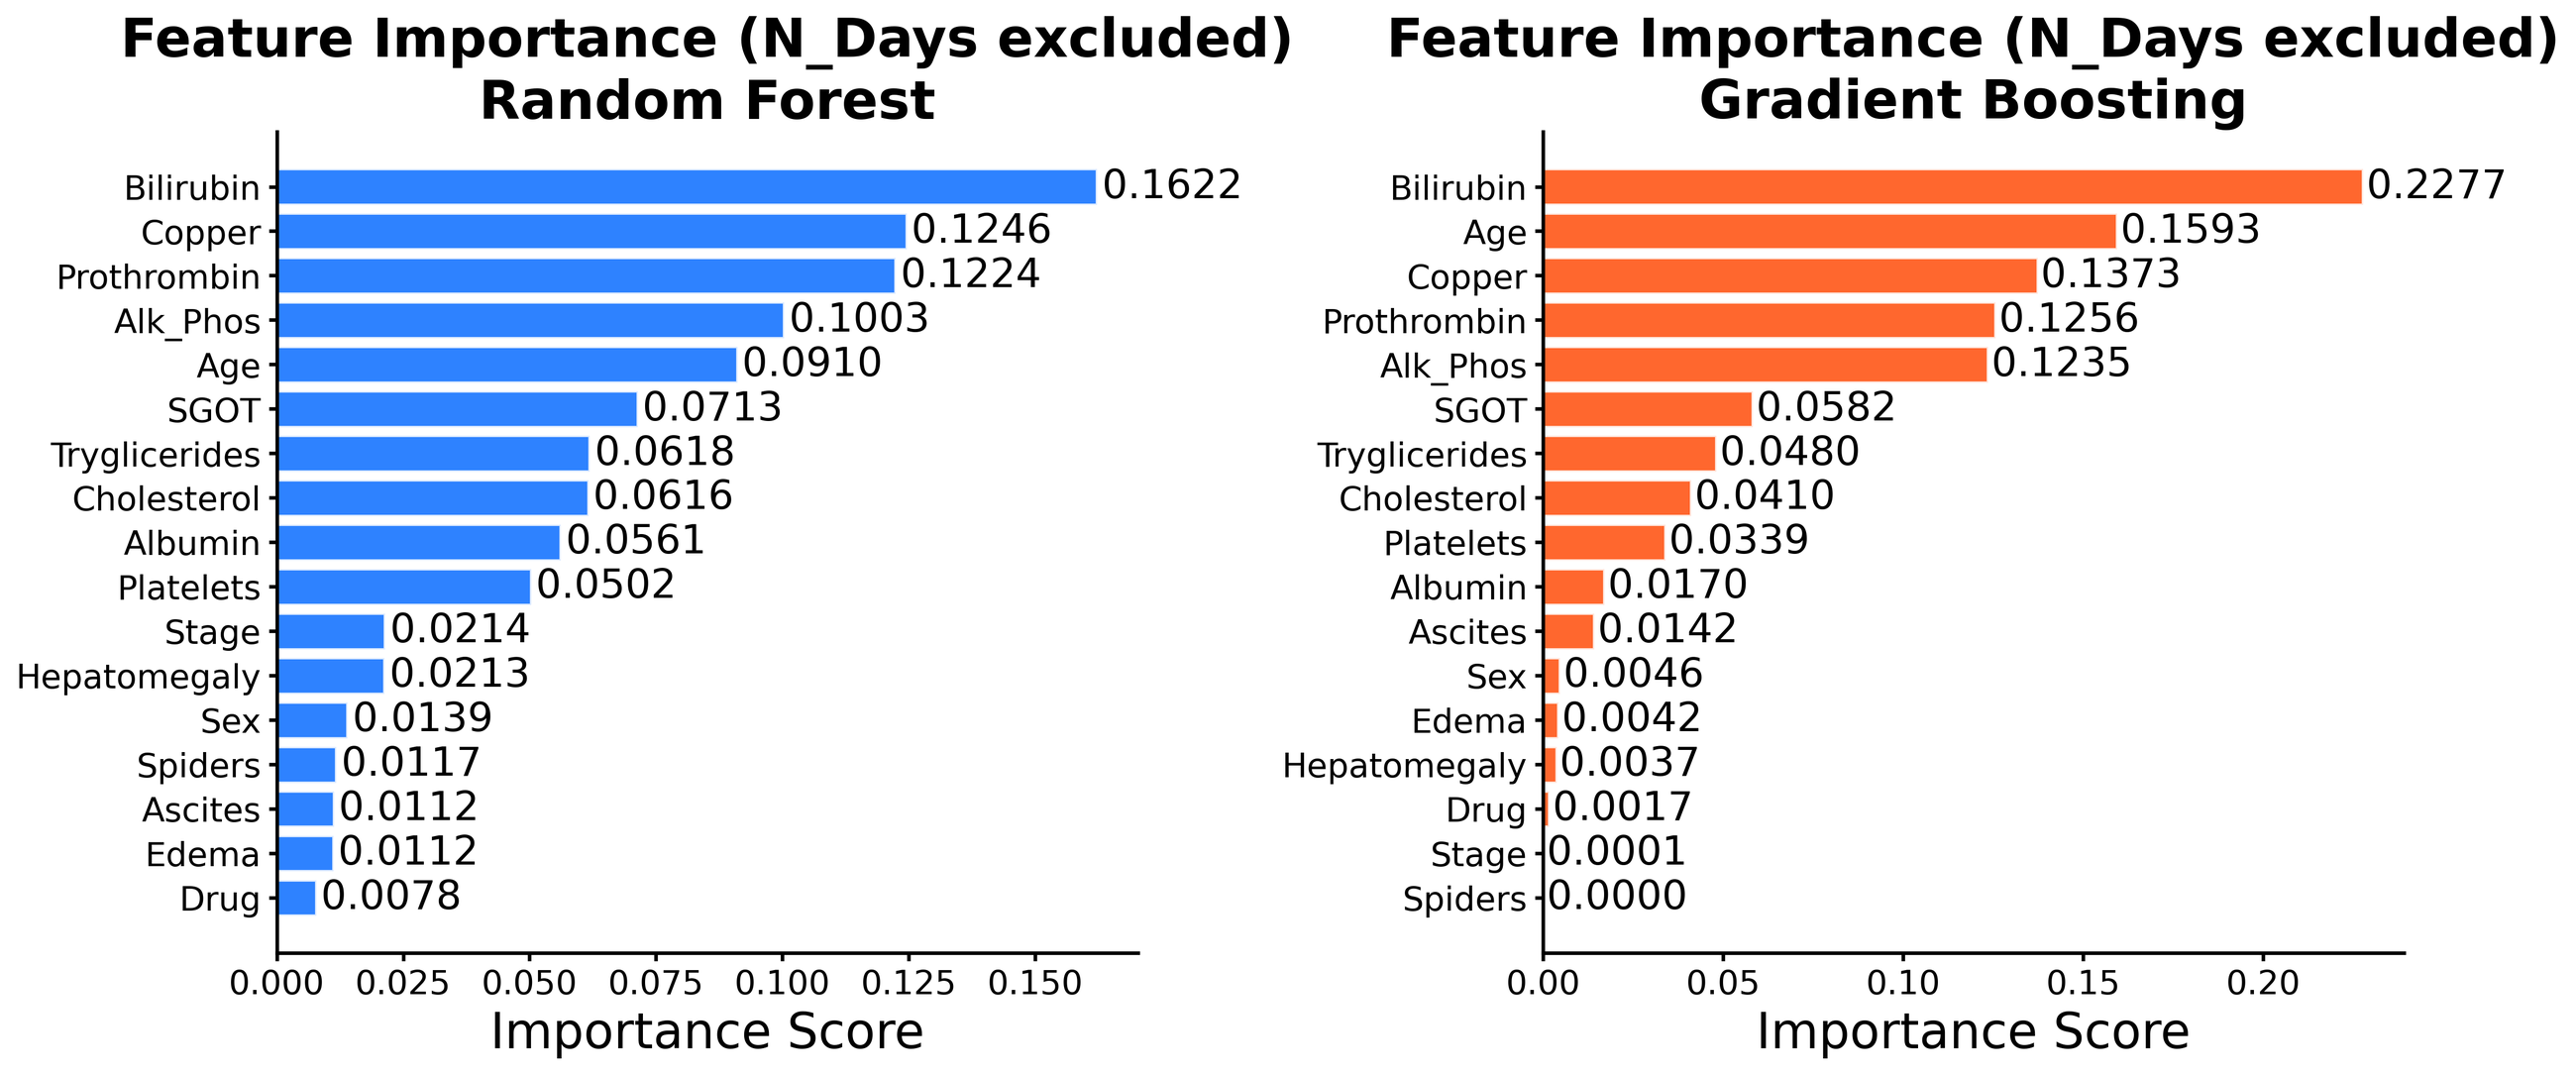
\includegraphics[width=0.98\textwidth]{fig07_feature_importance.png}
  \caption{Feature importance rankings from Random Forest (left) and Gradient Boosting (right) trained on real data only under Scenario A, N\_Days excluded from the input. Bilirubin leads both classifiers (RF 0.162, GB 0.228), followed by Copper, Prothrombin, and Alkaline Phosphatase; Gradient Boosting also weights Age highly (0.159). Binary clinical indicators show comparatively low importance, consistent with the dominant role of laboratory measurements in PBC prognosis.}
  \label{fig:importance}
\end{figure*}

\subsection{Fixed-Horizon Landmark Classification Results}
\label{sec:landmarkresults}

Table~\ref{tab:landmark} reports Scenarios A-E under the 3-year landmark framing (Section~\ref{sec:landmark}). 187 of the 193 real training patients and 76 of the 83 real test patients are usable, with an event rate of 17.1\% in training and 25.0\% in test, both well below the 40.4\% "ever deceased" rate used in the main classification framing. AUCs are higher across the board than in Table~\ref{tab:performance}, including for the baseline, where Logistic Regression reaches 0.916. This fits a fixed-horizon task simply being easier to discriminate than an unbounded one; it is not evidence of a stronger augmentation effect. We computed bootstrap confidence intervals (95\%, 1000 resamples) and McNemar's exact test against the baseline for all three augmentation scenarios this time, B, C, and D, not only the two deep-generative ones. Scenario B's Random Forest AUC of 0.908 [0.810, 0.981] and Scenario C's 0.910 [0.807, 0.984] both edge out the baseline's 0.892 [0.774, 0.975], while SMOTE (Scenario D) does not, at 0.874 [0.753, 0.967]. But the intervals are wide at this smaller sample size and overlap heavily in every case. McNemar's test finds no significant difference anywhere, including for SMOTE ($p$ ranges from 0.453 to 1.000 across all nine classifier-scenario pairs). So the landmark framing reaches the same conclusion as the main classification framing, augmentation gives no statistically distinguishable improvement, while also avoiding the coarser censoring problem the reviewer raised.

\begin{table}[!tb]
  \centering
  \caption{Landmark Classification Performance, 3-Year Horizon (76 Real Held-Out Patients)}
  \label{tab:landmark}
  \resizebox{\columnwidth}{!}{%
  \begin{tabular}{llccc}
    \toprule
    Scenario & Classifier & $n_{\text{train}}$ & Accuracy & AUC \\
    \midrule
    A: Baseline       & Random Forest      & 187 & 0.8158 & 0.8924 \\
    A: Baseline       & Gradient Boosting  & 187 & 0.8289 & 0.8356 \\
    A: Baseline       & Logistic Regression& 187 & 0.8684 & \textbf{0.9160} \\
    \midrule
    B: Real + cGAN   & Random Forest      & 443 & 0.8421 & 0.9077 \\
    B: Real + cGAN   & Gradient Boosting  & 443 & 0.8289 & 0.8652 \\
    B: Real + cGAN   & Logistic Regression& 443 & 0.8816 & 0.9252 \\
    \midrule
    C: Real + Consensus & Random Forest    & 934 & 0.8289 & 0.9104 \\
    C: Real + Consensus & Gradient Boosting& 934 & 0.8421 & 0.8680 \\
    C: Real + Consensus & Logistic Regression & 934 & 0.8553 & 0.9077 \\
    \midrule
    D: Real + SMOTE   & Random Forest      & 310 & 0.8553 & 0.8740 \\
    D: Real + SMOTE   & Gradient Boosting  & 310 & 0.7895 & 0.8246 \\
    D: Real + SMOTE   & Logistic Regression& 310 & 0.8289 & 0.9040 \\
    \midrule
    E: Synthetic Only (cGAN) & Random Forest      & 256 & 0.8553 & 0.9100 \\
    E: Synthetic Only (cGAN) & Gradient Boosting  & 256 & 0.8158 & 0.8901 \\
    E: Synthetic Only (cGAN) & Logistic Regression& 256 & 0.9079 & 0.8957 \\
    \bottomrule
  \end{tabular}%
  }
\end{table}

Extending Scenario E to all six generators under this framing turns up something the classification framing never showed: the VAE's synthetic pool collapses to a single class after landmark filtering, for every classifier, so we report it as missing rather than a crash (Section~\ref{sec:predutil}). In plain terms, the VAE's generated N\_Days and Status pairs do not land on both sides of the 3-year mark in this sample, one more sign of the over-smoothing already visible in its FID and KS statistics. The other five generators still work fine, and, as in the main classification framing, show no consistent link between distributional fidelity and landmark AUC.

\subsection{Time-to-Event Survival Modelling Results}
\label{sec:survivalresults}

Table~\ref{tab:survival} reports Scenarios A-E under the Cox/Random-Survival-Forest framing (Section~\ref{sec:survival}), using each patient's full follow-up time rather than a fixed horizon. The baseline C-index is 0.861 for both Cox and RSF, close to the classification framing's baseline AUC once N\_Days is excluded, which tells us that discarding censoring information was not itself hiding a lot of extra signal. No augmentation scenario improves on the Cox C-index: cGAN, consensus, and the SMOTE analog from Section~\ref{sec:survival} all sit at or below the baseline of 0.861 (0.860, 0.847, and 0.850). The Random Survival Forest is more mixed: cGAN and consensus again sit at or below baseline (0.858 and 0.855 against 0.861), but the SMOTE analog nominally comes out ahead, at 0.867. We did not run a significance test on the C-index, so read this single number the same way as the SMOTE result in the classification framing, a nominal gain we cannot yet confirm, not a contradiction of the null result that holds everywhere else.

\begin{table}[!tb]
  \centering
  \caption{Survival Modelling Performance: Harrell's C-Index (83 Real Held-Out Patients)}
  \label{tab:survival}
  \begin{tabular}{lccc}
    \toprule
    Scenario & $n_{\text{train}}$ & C-index (Cox) & C-index (RSF) \\
    \midrule
    A: Baseline          & 193 & 0.8606 & \textbf{0.8612} \\
    B: Real + cGAN      & 485 & \textbf{0.8601} & 0.8584 \\
    C: Real + Consensus  & 980 & 0.8470 & 0.8549 \\
    D: Real + SMOTE-analog & 230 & 0.8498 & 0.8669 \\
    E: Synthetic Only (cGAN) & 292 & 0.8385 & 0.8629 \\
    \bottomrule
  \end{tabular}
\end{table}

\subsection{Discussion}

None of the augmentation scenarios gave a statistically significant improvement on the 83-patient held-out test set. Once we take N\_Days out of the classifier's input, the real-data baseline is clearly weaker than it first looked: the earlier reported AUC of 0.878 for Gradient Boosting depended on a feature that leaks the outcome. The leak-free baseline now peaks at 0.842 for Logistic Regression, with Gradient Boosting down to 0.830. This reopens some of the headroom our original analysis argued was mostly gone, and the two deep-generative scenarios do move a little in both directions depending on the scenario and classifier (Table~\ref{tab:performance}). But none of that movement is distinguishable from noise (Table~\ref{tab:significance}). The PBC dataset still carries enough signal, even without N\_Days, for the classifiers to discriminate well, and the synthetic augmentation we tested does not move the decision boundary enough to change held-out predictions by a significant amount.

The cross-validation results back this up rather than overturn it. Repeating training across five folds, with synthetic data kept only on the training side, shows no augmentation scenario improving the mean AUC over baseline for Random Forest or Gradient Boosting. The fold-to-fold variance moves in no consistent direction either (Gradient Boosting goes from 0.0535 to 0.0480 between Scenario A and C; Random Forest goes the other way, from 0.0464 to 0.0532). An earlier version of this analysis let synthetic records into the validation folds and appeared to show a large drop in variance, but that was just an artefact: consensus records are drawn from the dense centre of feature space, so they are easier and more uniform to predict, and including them in validation mechanically shrinks the measured variance. Once validation is restricted to real patients, that apparent stability gain disappears, whether or not N\_Days is included. This is a warning worth stating plainly on its own: never evaluate synthetic augmentation on folds that themselves contain synthetic data.

\label{sec:power}
Fig.~\ref{fig:power} works out the statistical power of the McNemar test at this dataset size, using the discordant-pair counts we actually observed in Table~\ref{tab:significance} (a mean of 8 pairs, a 9.2\% discordant rate on $n=83$), rather than just assuming a rate. At this rate, the test has only 11\% power to detect a real 5-percentage-point accuracy gain. Reaching 80\% power at that effect size would need roughly 270 held-out patients. This does not undo the null result. Every McNemar p-value in this study, from 0.070 to 1.00, fell short of significance. But it does mean we cannot rule out a small real benefit. This needs replication on a larger cohort before we can say augmentation definitely does not help with this disease.

\begin{figure*}[!t]
  \centering
  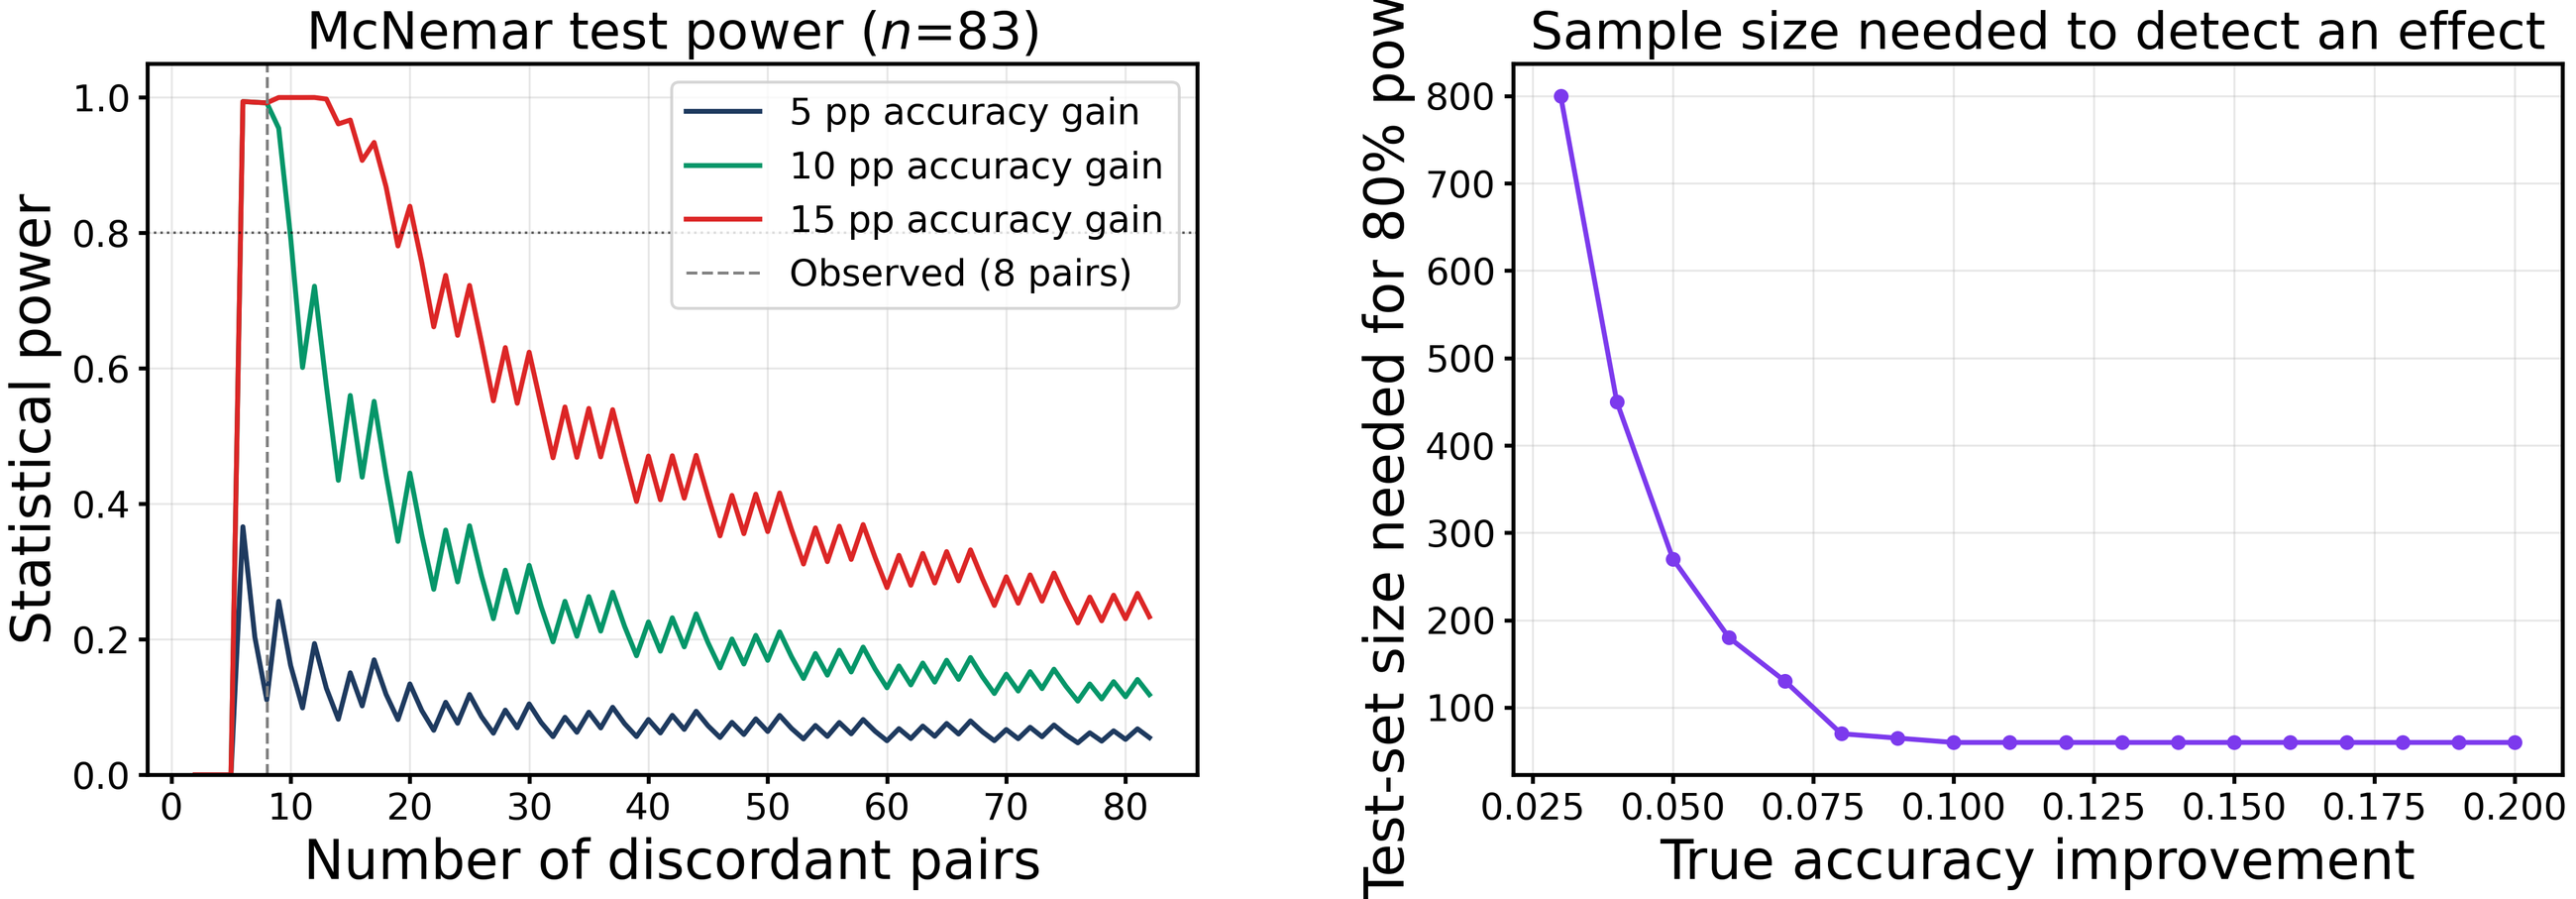
\includegraphics[width=0.98\textwidth]{fig08_power_analysis.png}
  \caption{Post-hoc power analysis for McNemar's exact test on 83 held-out patients, using the observed discordant-pair counts from Table~\ref{tab:significance}. Left: statistical power versus number of discordant pairs for three assumed accuracy gains; at the observed mean of 8 discordant pairs the test has 11\% power to detect a 5 percentage-point accuracy gain at $\alpha = 0.05$. Right: required test-set size for 80\% power versus true accuracy improvement, holding the observed 9.2\% discordant-pair rate fixed, showing that approximately 270 patients are needed for a 5-point gain.}
  \label{fig:power}
\end{figure*}

Scenario~E in Table~\ref{tab:performance} asks whether a classifier trained only on synthetic data can generalise to real patients, on the leak-free feature set. Using the 292 IQR-filtered cGAN records as the only training data, and the held-out 83 real patients as the test set, Logistic Regression discriminates best at AUC~$=0.849$, followed by Random Forest at AUC~$=0.809$. Gradient Boosting struggles much more without real data, falling to AUC~$=0.687$. Section~\ref{sec:sixgen} runs this same comparison across all six generators, which tells us whether this transfer is special to cGAN or holds for synthetic data more broadly.

Table~S8 of the supplementary document shows how consistent the results are across patient subgroups, on the leak-free 17-feature input. We trained classifiers under Scenario A and Scenario C and tested each separately on three clinically meaningful splits: disease stage (early Stage 1--2, $n=17$; late Stage 3--4, $n=66$), sex (female $n=72$; male $n=11$), and treatment arm (D-penicillamine $n=39$; placebo $n=44$). For the subgroups large enough to trust, late stage, female, and both treatment arms, AUC differences between Scenario A and C stayed within about $\pm0.04$ for every classifier, moved in no consistent direction, and every AUC stayed above 0.76. So the null result holds across the main clinical groups in this cohort, not just overall. The early-stage ($n=17$) and male ($n=11$) subgroups are too small to trust and swing around a lot; Random Forest AUC, for example, moves from 0.52 to 0.57 on the 11 male patients while Logistic Regression moves from 0.60 to 0.77 on the very same patients. We report them only for completeness. This still needs checking against an outside cohort.

The full VAE privacy-enhancement sweep is plotted in Fig.~S15 of the supplementary document (numeric values in Tables~S6 and~S7). This matters because consensus voting alone does not give a low-risk set either (21.1\% near-duplicates, Table~\ref{tab:privacy}). The filtered VAE pool of 499 records has a 35.7\% near-duplicate rate, so more than one in three generated records sits closer to a real training patient than the 5th-percentile real-to-real distance. To fix this without retraining the model, we added Gaussian noise to each VAE record's eleven continuous features after generation, scaled to each feature's training-data spread. At $\sigma=0.7$, the near-duplicate rate drops from 35.7\% to 1.4\%, and FID actually improves too, from 0.228 to 0.0481, better than the equalised consensus FID of 0.0809. That FID improvement looks strange at first, but makes sense: the VAE was clustering records too close to specific real patients, so spreading those clusters out brings its overall distribution closer to the real one. We also tried formal DP-SGD training across noise multipliers from 0.5 to 3.0, giving epsilon values between 14.0 and 210.4 at $\delta=10^{-5}$, far too large for any meaningful privacy guarantee. So output noise at $\sigma=0.7$ is the most practical fix at $n=193$. Formal differential privacy through DP-SGD only becomes realistic once a cohort reaches several hundred patients.

\subsection{Why Augmentation Did Not Improve Prediction}
\label{sec:whynot}

This null result deserves an explanation, not just a plain observation.

A generative model trained on the 193 real training patients is just a function of those patients plus some randomness. Whatever it produces is a transformation of information already sitting in the training set. By the data processing inequality, synthetic records cannot carry more information about the true population than the data they came from. Augmentation can reweight or smooth what the training data already shows, but it cannot add fresh evidence about patients the model never saw. That puts a hard ceiling on what augmentation can achieve, and on a cohort where the leak-free baseline classifier already reaches AUC~$=0.842$, there is not much headroom left beneath that ceiling, though more than the earlier analysis suggested when N\_Days had inflated the apparent baseline to 0.878.

The consensus mechanism actually works against itself here. Cross-architecture agreement, by design, only accepts records that all three models place in the same region of feature space, and that region is the dense centre of the training distribution. Our privacy results confirm this directly: the consensus set has a 21.1\% near-duplicate rate, higher than either adversarial pool, meaning its records sit unusually close to real patients. Records that close to existing training points are, almost by definition, redundant to a classifier. They reinforce parts of the feature space that are already well covered and add nothing near the decision boundary, the only place extra samples could actually change a fitted model.

This also explains why the effect differs by classifier. Random Forest and Gradient Boosting split feature space along axes, so points that fall inside an existing partition leave the split thresholds almost untouched. Logistic Regression fits one global boundary instead, so it is more sensitive to the extra probability mass, which is why it shows the largest movement across scenarios in Table~\ref{tab:performance}.

Scenario~E gives the clearest evidence for this reading. When synthetic data is the only training data, it is no longer competing against a stronger real signal, and it does reasonably well: AUC 0.81 to 0.85 for Random Forest and Logistic Regression. Synthetic data can substitute for real data that is missing, but it cannot add to real data that is already enough. That distinction, substitution rather than augmentation, is the practical lesson of this study.

\subsection{Scenario E Across Six Generators: Does FID Predict Utility?}
\label{sec:sixgen}

Our abstract's headline claim, that a synthetic dataset looking statistically similar to real data does not mean it is useful for prediction, used to rest on a single comparison: cGAN had the lowest FID among the three core generators and gave no augmentation benefit. That is one data point, not a correlation. Here we run Scenario~E (train-on-synthetic, test-on-real, leak-free 17-feature input) for all six generators in this study, so FID can be checked against downstream utility across more than one point, as the reviewer asked. CTGAN, built earlier but never wired into the evaluation pipeline until now, was trained for 4,000 epochs under the same seed-42 setup as every other generator, the same run reported in Section~\ref{sec:ctgancomp}. This is likely short of full convergence at this cohort size, a choice we made to keep training time bounded and reliable, so read the FID and TSTR results for CTGAN here as a partially-converged snapshot, not its best possible quality.

Table~\ref{tab:sixgen} lists each generator's FID next to the TSTR AUC of all three classifiers, and Fig.~\ref{fig:sixgen} plots FID against mean TSTR AUC. The relationship is weak and not significant: Pearson $r=0.35$ ($p=0.50$), Spearman $\rho=0.26$ ($p=0.62$) across the six generators. The masked-loss VAE has the best FID (0.062) and a strong mean TSTR AUC (0.798), which fits good utility. But the Vanilla GAN, with a middling FID (0.100), has the highest mean TSTR AUC of any generator (0.822), and the VAE, with by far the worst FID (0.228), still reaches a competitive mean TSTR AUC (0.812), because its Random Forest and Gradient Boosting results hold up even though its distributions do not. cGAN and CTGAN, with FID scores in the middle of the pack, actually have the two lowest mean TSTR AUCs (0.781 and 0.777). No steady relationship survives once a sixth generator joins the comparison. This six-point result is what our narrower abstract claim now rests on, not a guess from a single comparison.

\begin{table}[!tb]
  \centering
  \caption{FID and Train-on-Synthetic-Test-on-Real AUC Across Six Generators (Leak-Free 17-Feature Input, Status Target)}
  \label{tab:sixgen}
  \resizebox{\columnwidth}{!}{%
  \begin{tabular}{lccccc}
    \toprule
    Generator & FID & RF AUC & GB AUC & LR AUC & Mean AUC \\
    \midrule
    Vanilla GAN     & 0.0995 & 0.8258 & 0.8297 & 0.8115 & \textbf{0.8223} \\
    cGAN           & 0.0724 & 0.8091 & 0.6867 & 0.8485 & 0.7814 \\
    VAE            & 0.2280 & 0.8403 & 0.8152 & 0.7794 & 0.8116 \\
    Masked-loss VAE & \textbf{0.0619} & 0.8567 & 0.8036 & 0.7321 & 0.7975 \\
    CTGAN          & 0.1079 & 0.7997 & 0.7321 & 0.7994 & 0.7771 \\
    Consensus       & 0.0809 & 0.8336 & 0.7933 & 0.7867 & 0.8045 \\
    \bottomrule
  \end{tabular}%
  }
\end{table}

\begin{figure}[!tb]
  \centering
  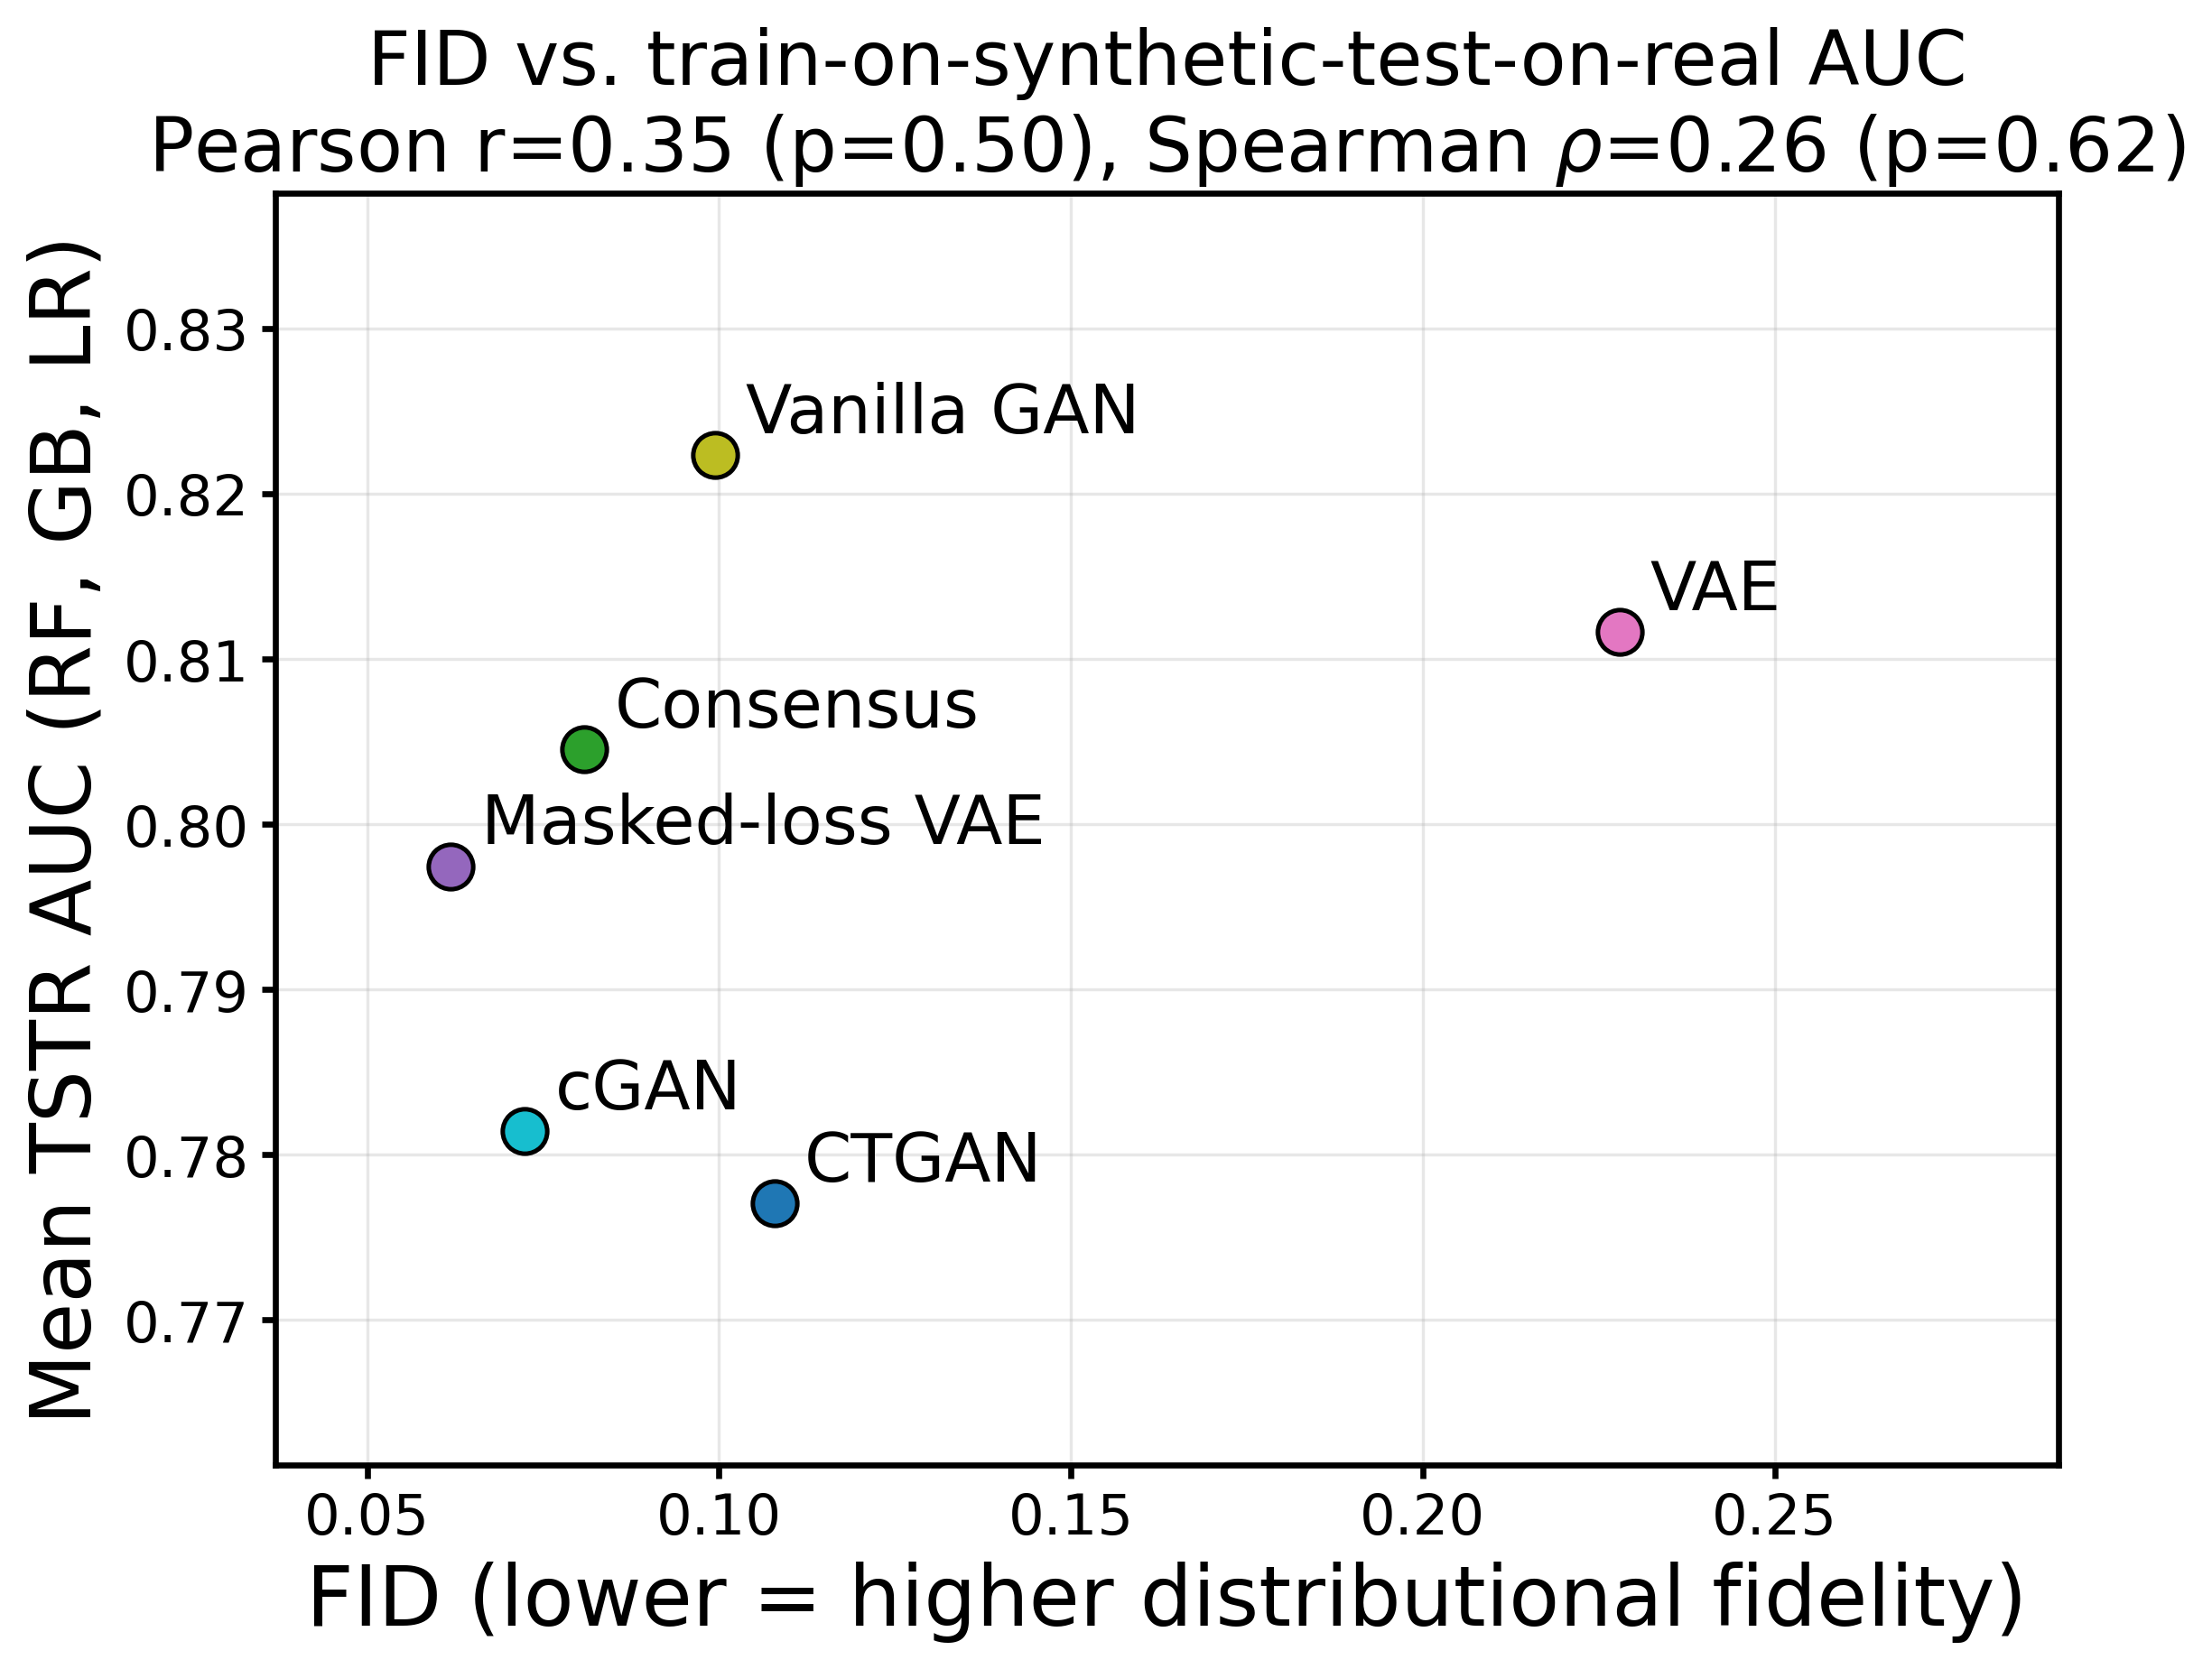
\includegraphics[width=\columnwidth]{fig11_fid_vs_tstr.png}
  \caption{FID versus mean train-on-synthetic-test-on-real AUC across all six generators in this study. Pearson $r = 0.35$ ($p = 0.50$), Spearman $\rho = 0.26$ ($p = 0.62$): neither correlation is statistically significant. The masked-loss VAE combines the best FID with strong utility, but the Vanilla GAN reaches the highest mean TSTR AUC from a middling FID, and the VAE reaches competitive utility from by far the worst FID.}
  \label{fig:sixgen}
\end{figure}

We can check this a second way, using the survival framing directly. We compared each generator's synthetic (N\_Days, Status) distribution against the real training cohort with Kaplan-Meier curves and a log-rank test (Section~\ref{sec:survival}); the full curves are given in Fig.~S12 of the supplementary document. The masked-loss VAE and cGAN reproduce the real survival curve closely (log-rank $p=0.773$ and $p=0.467$), the Vanilla GAN is borderline ($p=0.088$), while the VAE diverges sharply ($p=0.0006$), CTGAN diverges significantly ($p=0.038$), and even the consensus set, despite a mid-range FID of 0.081, diverges significantly too ($p=0.010$). This is the same point again from a different angle: FID is computed over the full 18-dimensional feature geometry, so it does not tell us on its own whether the time-to-event structure specifically is reproduced, and a generator can do well on one and badly on the other.

\subsection{Implications for Federated IoMT Deployment}
\label{sec:federated}

Scenario~E matters most for IoMT settings where hospitals cannot pool patient data. GDPR and HIPAA stop a hospital from exporting identifiable records, so a model that needs data from several sites cannot simply be trained on all of them together.

Our results show the records themselves may not need to move. One site can train a generator locally and release only synthetic records. A second site can then train a classifier on that output and still reach AUC 0.81 to 0.85 on its own real patients, without ever seeing a real record from the first site. This keeps disclosure risk low too: the filtered cGAN pool has a 9.6\% near-duplicate rate, and output perturbation brings the VAE's rate down from 35.7\% to 1.4\% where a stricter guarantee is needed. This approach also suits IoMT infrastructure well: it moves less data over constrained uplinks, lets the receiving site keep and reuse what it trains on, and reduces privacy governance to a one-time check on the synthetic set rather than ongoing per-record consent.

Two limits are worth stating plainly. Gradient Boosting fell to AUC~$0.687$ under Scenario~E, and this same weakness shows up for every generator we tested (mean TSTR AUC 0.777 to 0.822 across all six), so a receiving site must check its own choice of model rather than assume this transfers safely. And synthetic transfer is only worth doing where real data genuinely cannot be shared. Where pooling is allowed, Table~\ref{tab:performance} shows real data should just be used directly, since augmentation adds nothing once enough real records are already available.

\subsection{Comparison Against a Full CTGAN Implementation}
\label{sec:ctgancomp}

The conditional GAN in Section~\ref{sec:methodology} only borrows the conditioning idea from Xu et al.\ \cite{xu2019}, not their full architecture. To check what that simplification costs, we also built a full CTGAN with all three of its defining parts: mode-specific normalisation (a Gaussian mixture fitted per continuous column), a conditional vector with training-by-sampling, and a PacGAN critic trained with the Wasserstein gradient penalty. Full architecture details are in the supplementary material.

The simpler model still wins. Trained for 4,000 epochs (4,000 gradient updates, since this cohort size gives one step per epoch), CTGAN reached FID 0.108 against 0.072 for the conditional GAN, and only 40.8\% of its output passed the IQR filter against 58.4\%. This gap looks like a property of the small cohort rather than a flaw in CTGAN itself: 193 training rows gives very few gradient steps per epoch, so the epoch counts common in the CTGAN literature translate into far fewer real updates than usual, and 4,000 updates is likely short of convergence. We report the conditional GAN throughout the main analysis and name it accordingly. CTGAN is still included as a sixth generator in Section~\ref{sec:sixgen}'s comparison, at this same training budget.

\subsection{Threats to Validity}

Several things limit how far these findings generalise.

This is one cohort and one disease. PBC moves slowly and has strong, well-known biomarkers, so the baseline classifiers already have a lot to work with. A noisier disease, or one with weaker individual predictors, would likely leave augmentation more room to help.

Complete-case analysis dropped 142 of the 418 records. Patients 313 to 418 belong to an observational cohort where 9 or 10 lab measurements were simply never collected, so this exclusion follows trial protocol, not anything about the patients themselves. Our results describe the randomised trial population, and may not carry over to the observational arm.

Those 142 records still hold real, useful information. Every one of them has the survival outcome plus N\_Days, Bilirubin, and Albumin, which Fig.~\ref{fig:importance} ranks as the first, second, and fourth most important predictors. The missing data is not spread evenly either: 36 records are missing just one or two fields, while the other 106 are missing 9 or 10. So dropping all 142 throws away a fair amount of real, observed measurement, which is the most fixable limitation of this study, and we tested directly whether recovering it changes anything. As argued in Section~\ref{sec:whynot}, a generator trained only on the 193 complete records cannot know anything those records do not already contain. Records outside that set are real patients the generator never saw, so recovering them could, in principle, move the ceiling on what augmentation can do.

We trained a VAE whose reconstruction loss only counts the fields that were actually observed, so it can learn from partial records without imputing anything. This let it learn from 335 patients instead of 193, and it reached the best FID in the study, 0.062, better than the conditional GAN's 0.072. Augmenting the 193 real training patients with it gave the largest gain of any augmentation scenario we tested: AUC moved by $+0.035$, $+0.016$, and $-0.018$ for Random Forest, Gradient Boosting, and Logistic Regression (from a baseline of 0.832, 0.830, and 0.842 up to 0.868, 0.846, and 0.824). The Random Forest gain is the closest thing to a real effect anywhere in this study, six patients newly correct against only one newly wrong, but McNemar's test still falls short of significance ($p = 0.125$) and the bootstrap intervals still overlap. As Section~\ref{sec:power} explains, our test is simply underpowered to confirm an effect this size at $n=83$. That is not the same as evidence that no effect exists.

We ran two further checks using just the 36 same-protocol records (missing one or two fields, unlike the 106 observational records missing nine or ten). Adding these 36 directly after filling gaps with the median moved AUC by only $+0.004$, $+0.001$, and $+0.007$, noise-level changes, matching what the earlier, pre-correction analysis also found. But training a masked-loss VAE on the smaller 229-patient pool (193 real plus these 36) and augmenting with its output instead told a different story: Random Forest improved further, to $+0.010$, while Gradient Boosting and Logistic Regression fell, to $-0.016$ and $-0.031$. So passing real records through a generator is not simply worse than using them directly, as we had concluded before correcting the leak; it depends on the classifier, which fits the classifier-specific sensitivity already discussed in Section~\ref{sec:whynot}.

No scenario in this section overturns the paper's main null result at conventional significance. But the masked-loss VAE result is the one place where the size and direction of the effect, not just its sign, plausibly reflects something real: a modest, classifier-specific benefit from using more of the real signal we already have, through masked training rather than throwing partial records away.

A few smaller caveats. We left the classifiers at their default scikit-learn settings, apart from the tree counts stated in Section~\ref{sec:methodology}; tuning could move the baseline either way, and a weaker baseline would leave more room for augmentation to show a benefit, so we held capacity fixed across all five scenarios on purpose. The FID reported here is a tabular proxy on 18-dimensional feature vectors, not the image-domain FID from computer vision, so it is useful for ranking methods against each other here but not for comparing against FID values from other papers. The near-duplicate rate is a distance-based heuristic for privacy risk, not a formal guarantee; a record that sits far from every training patient in Euclidean space could still be identifiable through other information, and our DP-SGD analysis shows a formal privacy guarantee is out of reach at this sample size anyway. Our survival modelling (Section~\ref{sec:survival}) treats transplantation as censoring rather than as its own competing risk. Fig.~S11 suggests this is unlikely to bias the results much, since transplant makes up only 6.5\% of the cohort against 40.2\% for death, but confirming that properly would need a Fine-Gray model, which no package in our pipeline currently supports. Finally, our conditional GAN follows only the conditioning idea from Xu et al.\ \cite{xu2019}, not their full architecture, so it should not be read as a benchmark of cGAN as originally published.

\subsection{Practical Guidance for IoMT Deployments}

Four things follow for anyone building clinical decision support on a small tabular cohort like this one.

Never evaluate augmentation on validation folds that contain synthetic records. Our own earlier variance reduction disappeared completely once we restricted validation to real patients, so treat any stability gain measured on mixed folds as suspect until it survives a real-only check.

Judge synthetic data by what it does for held-out real patients, not by how well it matches the real distribution. Our conditional GAN had the best FID in the original three-model comparison and still gave no predictive benefit. FID and similar metrics describe how the data looks; only testing on real patients tells you whether it actually works.

Where synthetic data is genuinely needed, for cross-site sharing or when real records cannot leave a site, the conditional GAN is the safest choice here: lowest FID paired with a low near-duplicate rate. Do not release a VAE without extra care: ours reached a 35.7\% near-duplicate rate, which output noise at $\sigma=0.7$ brings down to 1.4\% while also improving FID.

Do not assume synthetic-only training works the same way across model families. Random Forest and Logistic Regression held AUC above 0.80 with no real training data at all, but Gradient Boosting fell to 0.687, and this same pattern showed up for all six generators, not just cGAN. Any deployment that trains on synthetic data should check its own choice of model before trusting the result.

% ---------------------------------------------------------------
% Section V: Conclusion
% ---------------------------------------------------------------
\section{Conclusion}
\label{sec:conclusion}

This paper set out to find what synthetic patient data can and cannot do for predicting liver cirrhosis survival in an IoMT setting. During peer review of an earlier version, we found that N\_Days, the follow-up duration used to work out Status, had been used as a classifier input. Since it leaks outcome information, this had inflated the reported baseline AUC from 0.842 to 0.878. Every result here now uses a 17-feature leak-free input. We also test the problem two further ways that avoid the cruder step of simply discarding censoring: fixed-horizon landmark classification, and full Cox/Random-Survival-Forest time-to-event modelling. We also extended the synthetic-only (Scenario E) evaluation from one generator to all six generators available in this study.

The corrected picture is more nuanced than our original one. With the leak removed, the real-data baseline is weaker than first reported, which reopens some real headroom. The two core deep-generative augmentation scenarios still cannot close that gap at statistical significance under any framing we tested (classification, landmark, or survival). But a masked-loss VAE trained on 335 partially observed patients, rather than the usual 193 complete cases, comes closest to a real effect in this study (Random Forest AUC $+0.035$, $p=0.125$). This points to recovering discarded partial records as a more promising direction than any of the generative-augmentation strategies we tested. Across all six generators, FID does not reliably predict train-on-synthetic-test-on-real utility (Pearson $r=0.35$, $p=0.50$; Spearman $\rho=0.26$, $p=0.62$): the masked-loss VAE pairs the best FID with strong utility, but the Vanilla GAN reaches the highest utility from a middling FID, and the VAE reaches competitive utility from the worst FID of any generator we tested. Synthetic data substitutes for real data that is unavailable, rather than adding to real data that is already enough. That distinction, together with the evidence that distributional fidelity does not predict utility, is what this study contributes.

We trained three generative models from scratch, under fixed random seeds, on the Mayo Clinic PBC dataset, plus a masked-loss VAE trained on a larger partially observed pool and a full CTGAN implementation. An IQR filter discarded roughly 34\% to 59\% of generated records across the six generators for being clinically implausible. A consensus voting step then kept only records that all three core architectures agreed on, giving an equalised set of 787 records.

Our main findings are these. The masked-loss VAE gave the best distributional quality, FID~$=0.062$, just ahead of cGAN at 0.072, and the filtered adversarial pools carried the lowest disclosure risk (7.3\% near-duplicates for GAN, 9.6\% for cGAN). No augmentation scenario beat the leak-free real-data baseline by a significant margin on the 83-patient test set, under any of the three framings. SMOTE nominally beat the baseline's Random Forest cross-validation mean (0.856 versus 0.850) but not by a significant margin, matching exactly the pattern the reviewer flagged in the pre-correction analysis. Consensus voting did not lower disclosure risk either, staying at 21.1\% near-duplicates, and its synthetic survival curve differs significantly from the real one ($p=0.010$ by log-rank test) despite a mid-range FID, one more sign that FID alone does not capture everything about utility. Classifiers trained only on synthetic cGAN data, with no real patients at all, still reached AUC 0.81 to 0.85 for Random Forest and Logistic Regression on real held-out patients (Gradient Boosting fell to 0.69, a pattern that held across all six generators). This confirms synthetic data carries real, though model-dependent, predictive signal, useful for federated IoMT settings where patient data cannot cross sites.

Three limitations remain. McNemar's test is underpowered at $n=83$: roughly 270 held-out patients would be needed to detect a 5-point accuracy gain with 80\% power at the discordant-pair rate we actually observed, so a small real benefit cannot be ruled out. VAE near-duplicate risk falls from 35.7\% to 1.4\% with output noise at $\sigma=0.7$, but formal differential privacy through DP-SGD is not workable until the cohort grows to several hundred patients. The SMOTE-style method we used for the survival framing, interpolating duration together with covariates for the event class, is a documented departure from off-the-shelf SMOTE, not a separately validated method. Replicating this on a larger, multi-site hepatology dataset, and extending it to ongoing IoMT data streams, are the priorities for future work.

\subsection*{Supplementary Material}
A supplementary document accompanies this paper, containing sixteen figures and eight tables. The figures are cited in the text as Fig.~S1 to Fig.~S16: S1, the Pearson correlation matrix across all 276 complete cases; S2, training loss curves for all three generative models; S3, feature distribution comparisons for six representative clinical variables; S4, real versus consensus correlation structure; S5, a t-SNE projection of real and synthetic records; S6, Precision-Recall curves; S7, AUC across scenarios; S8, the F1-score heatmap; S9 and S10, grouped comparisons of all five evaluation metrics across scenarios; S11, the Aalen-Johansen competing-risks cumulative incidence of death versus transplant discussed in Section~\ref{sec:survival}; S12, the Kaplan-Meier survival curves for all six generators against the real cohort discussed in Section~\ref{sec:sixgen}; S13, the IQR filtering effect on the Bilirubin distribution; S14, the privacy risk violin plots; S15, the VAE privacy-enhancement sweep; and S16, the end-to-end pipeline overview. Every quantity plotted in S6 to S10 also appears numerically in Tables~\ref{tab:performance} and~\ref{tab:cv}.

Tables~S1 to~S8 of that document report material omitted here for space: the complete architecture and optimiser settings for all three generative models; per-feature Kolmogorov-Smirnov statistics, Jensen-Shannon divergences and Cohen's $d$ for all eleven continuous features across all four synthetic datasets; the full consensus tolerance sweep across eight values; the output-perturbation and DP-SGD privacy sweeps; and the complete subgroup breakdown. Two results there are worth noting. The consensus set records the smallest KS statistics of any method on the hardest biomarkers despite being formally significant on all eleven features, and Cohen's $d$ ranks the VAE as the best-matched method on every feature even though it is the worst on every distributional-shape measure, which is a further instance of the paper's central point that a single fidelity metric can be satisfied by a model that is wrong in every other respect. The supplementary document and figures are distributed with the code repository.

\subsection*{Ethics Statement}
This study used the Mayo Clinic PBC dataset, which is publicly available, fully de-identified, and distributed for research use through the UCI Machine Learning Repository \cite{ucipbc}. No new patient data were collected and no additional ethical approval was required.

\subsection*{Data and Code Availability}
The Mayo Clinic PBC dataset is publicly available from the UCI Machine Learning Repository \cite{ucipbc}. All generative models, filtering and consensus code, and evaluation scripts are implemented in Python and TensorFlow~2.15 and run under fixed random seeds (Python, NumPy, and TensorFlow all seeded at 42), so the full pipeline, including synthetic data generation, reproduces the numbers reported here when re-executed in the same software environment. The survival-modelling framing additionally uses \texttt{lifelines} for Cox proportional-hazards fitting and, where available, \texttt{scikit-survival} for the Random Survival Forest. Because TensorFlow does not guarantee bitwise-identical arithmetic across different hardware or thread configurations, small numerical differences are possible on other systems. The code is available at https://github.com/Michaeludousoro/liver-cirrhosis-synthetic-data.

\subsection*{Declaration of Generative AI Use}
The authors used a generative AI assistant for code review, debugging, language editing, and, in response to peer review, implementing the corrected leak-free feature set, the landmark and survival-modelling framings, the six-generator extension of Scenario E, and the resulting pipeline reruns and analysis code described in this paper. All experiments, results, and scientific conclusions were verified by the authors against the underlying code and data, who take full responsibility for the content of this paper.

% ---------------------------------------------------------------
% References
% ---------------------------------------------------------------
\begin{thebibliography}{99}

\bibitem{guo2021}
A. Guo, N.~R. Mazumder, D.~P. Ladner, and R.~E. Foraker, ``Predicting mortality among patients with liver cirrhosis in electronic health records with machine learning,'' \textit{PLoS ONE}, vol.~16, no.~8, p.~e0256428, Aug.~2021, doi:~10.1371/journal.pone.0256428.

\bibitem{obeid2023}
J.~S. Obeid, A. Khalifa, B. Xavier, H. Bou-Daher, and D.~C. Rockey, ``An AI approach for identifying patients with cirrhosis,'' \textit{J. Clin. Gastroenterol.}, vol.~57, no.~1, pp.~82--88, Jul.~2021, doi:~10.1097/mcg.0000000000001586.

\bibitem{kanwal2020}
F. Kanwal \textit{et al.}, ``Development, validation, and evaluation of a simple machine learning model to predict cirrhosis mortality,'' \textit{JAMA Netw. Open}, vol.~3, no.~11, p.~e2023780, Nov.~2020, doi:~10.1001/jamanetworkopen.2020.23780.

\bibitem{goncalves2020}
A. Goncalves, P. Ray, B. Soper, J. Stevens, L. Coyle, and A.~P. Sales, ``Generation and evaluation of synthetic patient data,'' \textit{BMC Med. Res. Methodol.}, vol.~20, no.~1, p.~108, May~2020, doi:~10.1186/s12874-020-00977-1.

\bibitem{gonzales2023}
A. Gonzales, G. Guruswamy, and S.~R. Smith, ``Synthetic data in health care: A narrative review,'' \textit{PLoS Digit. Health}, vol.~2, no.~1, p.~e0000082, Jan.~2023, doi:~10.1371/journal.pdig.0000082.

\bibitem{yan2022}
C. Yan \textit{et al.}, ``A multifaceted benchmarking of synthetic electronic health record generation models,'' \textit{Nat. Commun.}, vol.~13, no.~1, p.~7609, Dec.~2022, doi:~10.1038/s41467-022-35295-1.

\bibitem{nikolentzos2023}
G. Nikolentzos, M. Vazirgiannis, C. Xypolopoulos, M. Lingman, and E.~G. Brandt, ``Synthetic electronic health records generated with variational graph autoencoders,'' \textit{NPJ Digit. Med.}, vol.~6, no.~1, p.~83, Apr.~2023, doi:~10.1038/s41746-023-00822-x.

\bibitem{che2017}
Z. Che, Y. Cheng, S. Zhai, Z. Sun, and Y. Liu, ``Boosting deep learning risk prediction with generative adversarial networks for electronic health records,'' in \textit{Proc. IEEE Int. Conf. Data Min.}, 2017, pp.~787--792, doi:~10.1109/icdm.2017.93.

\bibitem{kababji2023}
S.~E. Kababji \textit{et al.}, ``Evaluating the utility and privacy of synthetic breast cancer clinical trial data sets,'' \textit{JCO Clin. Cancer Inform.}, no.~7, p.~e2300116, Sep.~2023, doi:~10.1200/cci.23.00116.

\bibitem{espinosa2023}
E. Espinosa and A. Figueira, ``On the quality of synthetic generated tabular data,'' \textit{Mathematics}, vol.~11, no.~15, p.~3278, Jul.~2023, doi:~10.3390/math11153278.

\bibitem{guillaudeux2023}
M. Guillaudeux \textit{et al.}, ``Patient-centric synthetic data generation, no reason to risk re-identification in biomedical data analysis,'' \textit{NPJ Digit. Med.}, vol.~6, no.~1, p.~37, Mar.~2023, doi:~10.1038/s41746-023-00771-5.

\bibitem{kumari2024}
C. Kumari and R. Siddharthan, ``MMM and MMMSynth: Clustering of heterogeneous tabular data, and synthetic data generation,'' \textit{PLoS ONE}, vol.~19, no.~4, p.~e0302271, Apr.~2024, doi:~10.1371/journal.pone.0302271.

\bibitem{figueira2022}
A. Figueira and B. Vaz, ``Survey on synthetic data generation, evaluation methods and GANs,'' \textit{Mathematics}, vol.~10, no.~15, p.~2733, Aug.~2022, doi:~10.3390/math10152733.

\bibitem{vega2020}
B. Vega-M\'{a}rquez, C. Rubio-Escudero, and I. Nepomuceno-Chamorro, ``Generation of synthetic data with conditional generative adversarial networks,'' \textit{Log. J. IGPL}, vol.~30, no.~2, pp.~252--262, Nov.~2020, doi:~10.1093/jigpal/jzaa059.

\bibitem{choi2017}
E. Choi, S. Biswal, B. Malin, J. Duke, W.~F. Stewart, and J. Sun, ``Generating multi-label discrete patient records using generative adversarial networks,'' \textit{arXiv}, Mar.~2017, doi:~10.48550/arxiv.1703.06490.

\bibitem{lenz2021}
S. Lenz, M. Hess, and H. Binder, ``Deep generative models in DataSHIELD,'' \textit{BMC Med. Res. Methodol.}, vol.~21, no.~1, p.~64, Apr.~2021, doi:~10.1186/s12874-021-01237-6.

\bibitem{sharma2024}
D. Sharma, W. Lou, and W. Xu, ``PhylaGAN: Data augmentation through conditional GANs and autoencoders for improving disease prediction accuracy using microbiome data,'' \textit{Bioinformatics}, vol.~40, no.~4, p.~btae161, Apr.~2024, doi:~10.1093/bioinformatics/btae161.

\bibitem{meidan2018}
Y. Meidan \textit{et al.}, ``N-BaIoT: Network-based detection of IoT botnet attacks using deep autoencoders,'' \textit{IEEE Pervasive Comput.}, vol.~17, no.~3, pp.~12--22, Jul.~2018, doi:~10.1109/mprv.2018.03367731.

\bibitem{damico2023}
S. D'Amico \textit{et al.}, ``Synthetic data generation by artificial intelligence to accelerate research and precision medicine in hematology,'' \textit{JCO Clin. Cancer Inform.}, no.~7, p.~e2300021, Jun.~2023, doi:~10.1200/cci.23.00021.

\bibitem{kim2024}
H. Kim \textit{et al.}, ``Synthetic data improve survival status prediction models in early-onset colorectal cancer,'' \textit{JCO Clin. Cancer Inform.}, no.~8, p.~e2300201, Jan.~2024, doi:~10.1200/cci.23.00201.

\bibitem{tucker2020}
A. Tucker, Z. Wang, Y. Rotalinti, and P. Myles, ``Generating high-fidelity synthetic patient data for assessing machine learning healthcare software,'' \textit{NPJ Digit. Med.}, vol.~3, no.~1, p.~147, Nov.~2020, doi:~10.1038/s41746-020-00353-9.

\bibitem{dankar2022}
F.~K. Dankar, M.~K. Ibrahim, and L. Ismail, ``A multi-dimensional evaluation of synthetic data generators,'' \textit{IEEE Access}, vol.~10, pp.~11147--11158, Jan.~2022, doi:~10.1109/access.2022.3144765.

\bibitem{foraker2020}
R.~E. Foraker \textit{et al.}, ``Spot the difference: Comparing results of analyses from real patient data and synthetic derivatives,'' \textit{JAMIA Open}, vol.~3, no.~4, pp.~557--566, Dec.~2020, doi:~10.1093/jamiaopen/ooaa060.

\bibitem{kaabachi2023}
B. Kaabachi \textit{et al.}, ``A scoping review of privacy and utility metrics in medical synthetic data,'' \textit{medRxiv}, Nov.~2023, doi:~10.1101/2023.11.28.23299124.

\bibitem{jiang2023}
X. Jiang, J. Zheng, X. Zhuang, and Z. Ge, ``Ensemble data augmentation for imbalanced fault diagnosis,'' \textit{IEEE Trans. Instrum. Meas.}, vol.~72, pp.~1--12, Jan.~2023, doi:~10.1109/tim.2023.3307757.

\bibitem{pandey2025}
C. Pandey, V. Tiwari, S.~A.~J. Francis, V. Pal, and D.~S. Roy, ``MF-CGAN: Multifeature conditional GAN for synthetic data generation in Internet of Medical Things,'' \textit{IEEE Internet Things J.}, vol.~12, no.~10, pp.~13469--13476, Mar.~2025, doi:~10.1109/jiot.2025.3554207.

\bibitem{fleming1991}
T.~R. Fleming and D.~P. Harrington, \textit{Counting Processes and Survival Analysis}. New York, NY, USA: Wiley, 1991.

\bibitem{ucipbc}
E. Dickson, P. Grambsch, T. Fleming, L. Fisher, and A. Langworthy, ``Cirrhosis patient survival prediction,'' UCI Machine Learning Repository, 1989, doi:~10.24432/C5R02G. [Online]. Available: https://archive.ics.uci.edu/dataset/878/cirrhosis+patient+survival+prediction

\bibitem{mirza2014}
M. Mirza and S. Osindero, ``Conditional generative adversarial nets,'' \textit{arXiv}, Nov.~2014, doi:~10.48550/arxiv.1411.1784.

\bibitem{xu2019}
L. Xu, M. Skoularidou, A. Cuesta-Infante, and K. Veeramachaneni, ``Modeling tabular data using conditional GAN,'' in \textit{Proc. Adv. Neural Inf. Process. Syst. (NeurIPS)}, 2019, pp.~7335--7345.

\end{thebibliography}

\end{document}
